Siehe tolle Daten in Tab. \ref{tab:impl:data}.

\begin{table}
    \centering
    \begin{tabular}{|lcc|}
    \hline
              & \textbf{Regular Customers} & \textbf{Random Customers} \\ \hline
    Age       & 20-40                      & \textgreater{}60          \\ \hline
    Education & university                 & high school               \\ \hline
    \end{tabular}
    \caption{Ein paar tabellarische Daten}
    \label{tab:impl:data}
\end{table}

\begin{figure}
    \centering
    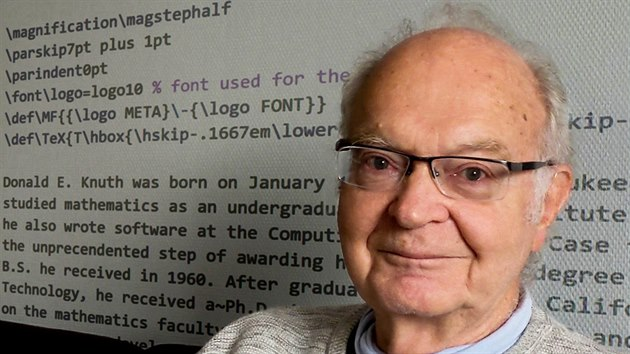
\includegraphics[scale=0.5]{pics/knuthi.jpg}
    \caption{Don Knuth -- CS Allfather}
    \label{fig:impl:knuth}
\end{figure}

Siehe und staune in Abb. \ref{fig:impl:knuth}.
\lipsum[6-9]
Dann betrachte den Code in Listing \ref{lst:impl:foo}.

\begin{lstlisting}[language=Python,caption=Some code,label=lst:impl:foo]
# Program to find the sum of all numbers stored in a list (the not-Pythonic-way)

# List of numbers
numbers = [6, 5, 3, 8, 4, 2, 5, 4, 11]

# variable to store the sum
sum = 0

# iterate over the list
for val in numbers:
    sum = sum+val

print("The sum is", sum)
\end{lstlisting}

\section{Plannung}

\subsection{Ideenfindung [M]}
\setauthor{Fabian Maar}
Die Ideenfindung ist der Start eines Projektes und bildet das Fundament, auf dem das Projekt entsteht. Die Idee für die Entstehung eines Projektes kann viele Motive haben, so ist es wichtig, als Projektteam diese zu erkennen und als Motivation zu nehmen. Während oder nach dem Prozess der Ideenfindungs wird schon bald klar, welche Projektwürdigkeit das Projekt besitzt. Somit kann schon frühzeitig entschieden werden, ob es sinnvoll erscheint, das Projekt zu realisieren oder ob nochmals eine neue Ideenfindung von Nöten ist. Auch bei dieser Diplomarbeit wurde der Prozess der Ideenfindung mehrmals wiederholt, wodurch die Wichtigkeit und die Methodik der Findung von Ideen besonders bemerkbar wurde. Die Ideenfindung erfolgt meist mit Hilfe der Anwendung einer passenden Kreativitätstechnik.

Kreativitätstechniken sind vielseitig einzusetzen, werden aber häufig am Anfang eines Projektes angewandt. Sie sind besonders hilfreich, wenn ein rationales Problemlösen nicht zielführend erscheint. Sie helfen, Ziele, Lösungen und Risiken zu finden, evaluieren und festzulegen. Für die Diplomarbeit bot sich besonders die Kreativitätstechnik Brainstorming an, da durch sie viele verschiedene Ideen in kürzester Zeit gesammelt werden können.

Beim Brainstormen findet jede*r Teilnehmer*in zu einem bestimmten Thema so viele Ideen wie möglich. Das Brainstormen erfolgt in 2 Phasen. Zuerst werden alle Ideen niedergeschrieben und anschließend die Beste herausgefiltert. Aufgrund der Expertise der Betreuungslehrerinnen im Bereich 3D-Modellierung und aus eigenem Interesse, konnte sich relativ schnell auf das Thema \emph{eine Software mit 3D-Integration} geeinigt werden. Schlussendlich konnte sich für eine Idee entschieden werden, nachdem das Brainstormen nach folgenden Kriterien erfolgt hat:
\begin{itemize}
    \item Quantität vor Qualität
    \item Freies Assoziieren und Fantasieren sind erwünscht
    \item Keine Kritik, Korrektur oder Meinungsäußerung
    \item Möglichst viele Ideen
    \item Inspirieren lassen von anderen
\end{itemize}
\cite{Ideenfindung}

\subsection{User-Stories}
\setauthor{Litzlbauer Lorenz}


\subsubsection{Projekt User Stories}
\setauthor{Team}
\begin{compactenum}
    \item Als Designer möchte ich einen Login, um meine Ausstellungen speichern und im nachhinein immer öffnen zu können.
    Akzeptanzkriterien: 
    \begin{compactitem}
        \item Man kann sich neu registrieren
        \item Registrierung mittels Username und Passwort
        \item Das Passwort muss überprüft werden beim Erstellen und mind. 8 Zeichen enthalten
    \end{compactitem}  
    \item Als erstmalige*r Besucher*in der Webseite möchte ich die benötigten Informationen über die Funktionen der Applikation verständlich erkennen können. Auswahlkriterien: 
    \begin{compactitem}
        \item Auf der Landingpage befinden sich: 
        \begin{compactitem}
            \item Textstellen und Grafiken, die unser Projekt und die Funktionalitäten davon erklären
            \item Einen Call-to-Action(CTA)-Button, der den User*in dazu einlädt, seine eigene Ausstellung zu erstellen. Beim Betätigen wird der Benutzer, falls er schon eingeloggt ist, weitergeleitet zum Editor, sonst zur Login Seite (hier gibt es die Möglichkeit, sich auch einen Account zu erstellen)
        \end{compactitem}
    \end{compactitem} 
    \item Als Besucher*in möchte ich eine Suchseite haben, um Designer*innen und deren Ausstellungen finden zu können. Auswahlkriterien: 
    \begin{compactitem}
        \item CTA-Search Field
        \item Eine Unterseite, welche durch den CTA-Button aufgerufen wird und unterschiedliche Optionen zur Verfügung stellt und das Suchergebnis ansprechend darstellt
    \end{compactitem} 
    \item  Als Besucher*in der Webseite, will ich beim Suchen filtern können, um für sich die relevantesten Ergebnisse zu bekommen. Auswahlkriterien: 
    \begin{compactitem}
        \item filtern über …
        \begin{compactitem}
            \item Tags
            \item Favoriten
            \item Erstellungsdatum
        \end{compactitem}
    \end{compactitem} 
    \item Als Benutzer*in möchte ich meinen Ausstellungen Tags zuordnen können, damit diese leichter gefunden werden können. Auswahlkriterien: 
    \begin{compactitem}
        \item Tags werden beim erstellen der Ausstellung aus einen vordefinierten Tag-Pool ausgewählt.
    \end{compactitem} 
    \item Als User*in möchte ich mich auf verschiedene Arten in der Ausstellung bewegen können. Auswahlkriterien: 
    \begin{compactitem}
        \item Per Slideshow (über den Vorwärts/Rückwärts-Pfeil zu nächstem Ausstellungsstück springen)
        \item Per Touch / Click (Google Maps Street View, NavigationMesh in Three.js https://github.com/donmccurdy/three-pathfinding)
    \end{compactitem} 
    \item  Als User*in möchte ich auf das Ausstellungsstück klicken können, um weitere Informationen (z.B.: Titel, Künstler, Jahr, …) zu erhalten. Auswahlkriterien: 
    \begin{compactitem}
        \item größere Ansicht des Ausstellungsstücks wird vergrößert angezeigt
        \item Nähere Details zum Ausstellungsstück, wie Titel, Künstler, Jahr, usw.
    \end{compactitem} 
    \item  Als User*in will ich eine Profil-Unterseite haben, auf der ich userrelevante Informationen angezeigt bekomme. Auswahlkriterien: 
    \begin{compactitem}
        \item userrelevante Informationen, die angezeigt werden, sind: 
        \item Name
        \item Profilfoto
        \item Erstellte Ausstellungen
        \item Der*Die User*in kann dort seine Ausstellungen löschen.         
    \end{compactitem} 
    \item  Als User*in will ich bei der Erstellung einer Ausstellung zwischen verschiedenen Templates wählen können, um diese auf einfache Weise zu individualisieren. Auswahlkriterien: 
    \begin{compactitem}
        \item Es gibt 2 Templates am Anfang, in denen die Wandfarbe, der Boden und die Podeste für die Dateien vorgegeben sind.
        \item Der*Die User*in kann keine Templates erstellen.
        \item Der*Die User*in kann manuell die Podeste für jede Datei zwischen 5 vorgefertigten auswählen und für den Boden + Wand ein Pattern hochladen
        \item Bei den Templates kann man aber manuell einzelne Aspekte verstellen (siehe Punkt oben)
    \end{compactitem} 
    \item Als User will ich meine Daten auf den Server laden, um diese jederzeit innerhalb einer Ausstellung platzieren und integrieren zu können. Auswahlkriterien: 
    \begin{compactitem}
        \item Unterstützte Dateien (Bilder-, Audio-, Video-, 3D-Dateien) 
        \item Uploadmöglichkeiten: 
        \begin{compactitem}
            \item Drag and Drop
            \item Im Ordner auswählen.
        \end{compactitem} 
        \item Dateigrößenlimit: 50MB
        \item Dateityp Limit: nur Standardformate (Bilder: JPG, PNG, etc.;        Audio: WAV, MP3, etc.; …)
        \item Fehlermeldung bei falschem Upload
    \end{compactitem} 
    \item  Als User*in will ich, dass meine Daten automatisch als Ausstellungsstücke in der Ausstellung angeordnet werden, damit die Nutzung für persönliche Bereiche unkompliziert möglich ist. Auswahlkriterien: 
    \begin{compactitem}
        \item Falls dies nicht möglich ist, soll eine Fehlermeldung angezeigt werden
    \end{compactitem} 
    \item Als User*in möchte ich die Reihenfolge und Platzierung meiner Werke innerhalb der Ausstellung adaptieren können. Auswahlkriterien: 
    \begin{compactitem}
        \item Die Werke sollen zwischen vordefinierten Plätzen tauschbar sein.
    \end{compactitem} 
    \item Als User*in will ich andere Rechte haben, je nachdem ich angemeldet bin oder nicht. Auswahlkriterien: 
    \begin{compactitem}
        \item Wenn ein*e User*in angemeldet ist, kann er*sie:
        \begin{compactitem}
            \item Ausstellungen ansehen 
            \item Ausstellungen erstellen/löschen 
            \item Ausstellungen favorisieren
        \end{compactitem}  
        \item Wenn ein ein*e User*in nicht angemeldet ist, kann er*sie: 
        \begin{compactitem}
            \item Ausstellungen ansehen 
            \item keine Ausstellungen erstellen 
            \item keine Ausstellungen favorisieren
        \end{compactitem} 
    \end{compactitem} 
    \item Als User*in möchte ich meine Ausstellung abspeichern und löschen können. Auswahlkriterien: 
    \begin{compactitem}
        \item Die Daten im Bezug auf die Ausstellungen werden auf dem Server gespeichert.
        \item Bevor die Ausstellung gelöscht wird, soll ein Warnhinweis angezeigt werden, welcher noch bestätigt werden muss. 
    \end{compactitem} 





\end{compactenum}

\subsection{fortlaufendes Prototyping}
\label{ch::ongoing-prototyping}

\section{Design}
\subsection{Userexperience [L]}
\setauthor{Litzlbauer Lorenz}
In keinem Softwareprojekt darf nicht der*die Benutzer*innen vergessen werden. Feature und Design müssen immer mit dem Gedanken entwickelt werden, wie hilft das dem*der Kunden*in oder der Zielgruppe weiter.

In den folgenden Kapiteln wird das Thema User Experience und wie dieses Thema im Projekt umgesetzt wurde, behandelt.
\subsubsection{UX Design (Userexperience)}
Ein gutes Userexperience-Design ist die Grundlage für eine erfolgreiche Positionierung und Kommunikation mit dem*der Benutzer*in.
UX bezieht sich dabei auf die Interaktion des Benutzers mit der Umwelt, aber auch mit dem angebotenen Service oder Produkt. In diesem Kontext hat Design mehrere Bedeutungen.
Erstens gibt es den Punkt der Gestaltung der Interaktionen, hierzu gehört der Begriff Interface Design (UI Design), er bedeutet visuelle Kommunikation über Zeichen und Symbole.
Zweitens gibt es Design als den Designprozess. Im Designprozess muss erkannt werden, was dem*der Benutzer*in wichtig ist und dieses dem Produkt zugewiesen werden, sodass es auch der*die Benutzer*in erkennen kann \cite{UserExperienceDesign}.

\subsubsection{Anwendungen von UX im Projekt}
Das Projekt wurde schon von Anfang an mit einem Gedanken für den Benutzer gestartet. Userstories waren aus der Sicht eines Benutzers formuliert und das Projekt startete mit der Frage, welchen Nutzen kann das Projekt einem*einer Nutzer*in geben.

Im Userinterface-Design wurde Figma (siehe Kapitel \hyperref[ch::technologies::figma]{Technologien Figma}) benutzt. Die Oberfläche wurde so designt, damit sie leicht verständlich, nützlich und benutzerfreundlich ist. Dafür wurden viele Prototypen (siehe Abbildung \ref{fig:impl:design:prototypesfigma}) in Figma gestallten und durch Umfragen die besten bestimmt und dementsprechende Anpassungen am Design gemacht.

\begin{figure}
    \centering
    \includegraphics[scale=0.3]{pics/ProjektOberflächenDesignPrototypenFigma.png}
    \caption{OberflächenDesign: Prototypen in Figma}
    \label{fig:impl:design:prototypesfigma}
\end{figure}

\subsection{Corporate Design [M]}
\setauthor{Fabian Maar}
Das Corporate Design unterstützt die Corporate Identity und deren Ziele. Unter der Corporate Identity versteht man das äußere Erscheinungsbild eines Unternehmens. Hierbei sollen Bestandteile eines Unternehmens nach außen hin einheitlich, unverwechselbar und positiv wirken und mit der Gesamtstrategie stimmig sein. Zum Beispiel werden Mitarbeiter, Abteilungen und Produkte sowie ihre Beziehungen zur Firma nach gewissen Normen strategisch gestaltet und geregelt. Dabei lässt sich die Corporate Identity in 3 Teilbereiche gliedern:

\begin{itemize}
    \item Corporate Behaviour
    \item Corporate Communication
    \item Corporate Design
\end{itemize}
\cite{CorporateIdentity}

Bei der Diplomarbeit kam vor allem das Corporate Design zum Einsatz. Hierbei wird vor allem das äußere Erscheinungsbild des Produkts als Einheit repräsentiert. Dabei werden zum Beispiel Hausfarbe, Logo, Gestaltungsraster und weitere Design-Elemente aufeinander abgestimmt. Dies war auch fester Bestandteil der Design-Phase.
\cite{CorporateDesign}

//TODO Text über Bild + Bilder richtig anordnen
Der erste Schritt des Designs war es, zwei unterschiedliche Konzepte der ersten Webseiten-Elemente zu erstellen. Anschließend wurden diese verglichen und sich für eines entschieden. Dieses erste Grundkonzept wurde das Grundgerüst für den späteren Verlauf der Designarbeit.

\begin{figure}
    \centering
    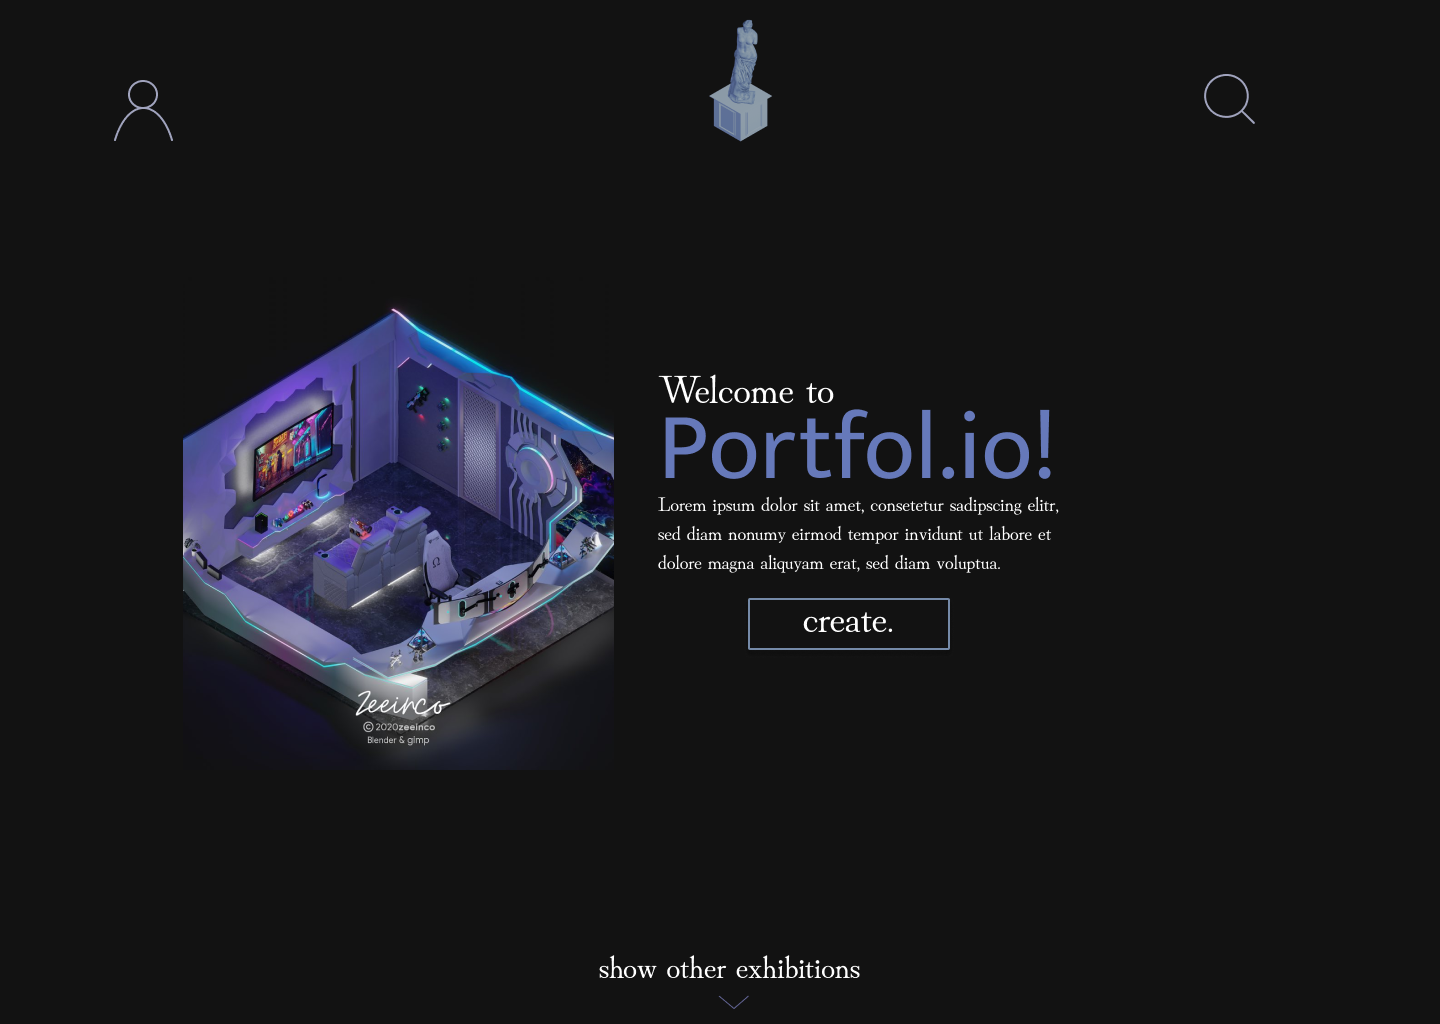
\includegraphics[scale=0.3]{pics/DesignKonzept1_1.png}
    \caption{Design Konzpet 1 Page 1}
    \label{fig:impl:knuth}
\end{figure}

\begin{figure}
    \centering
    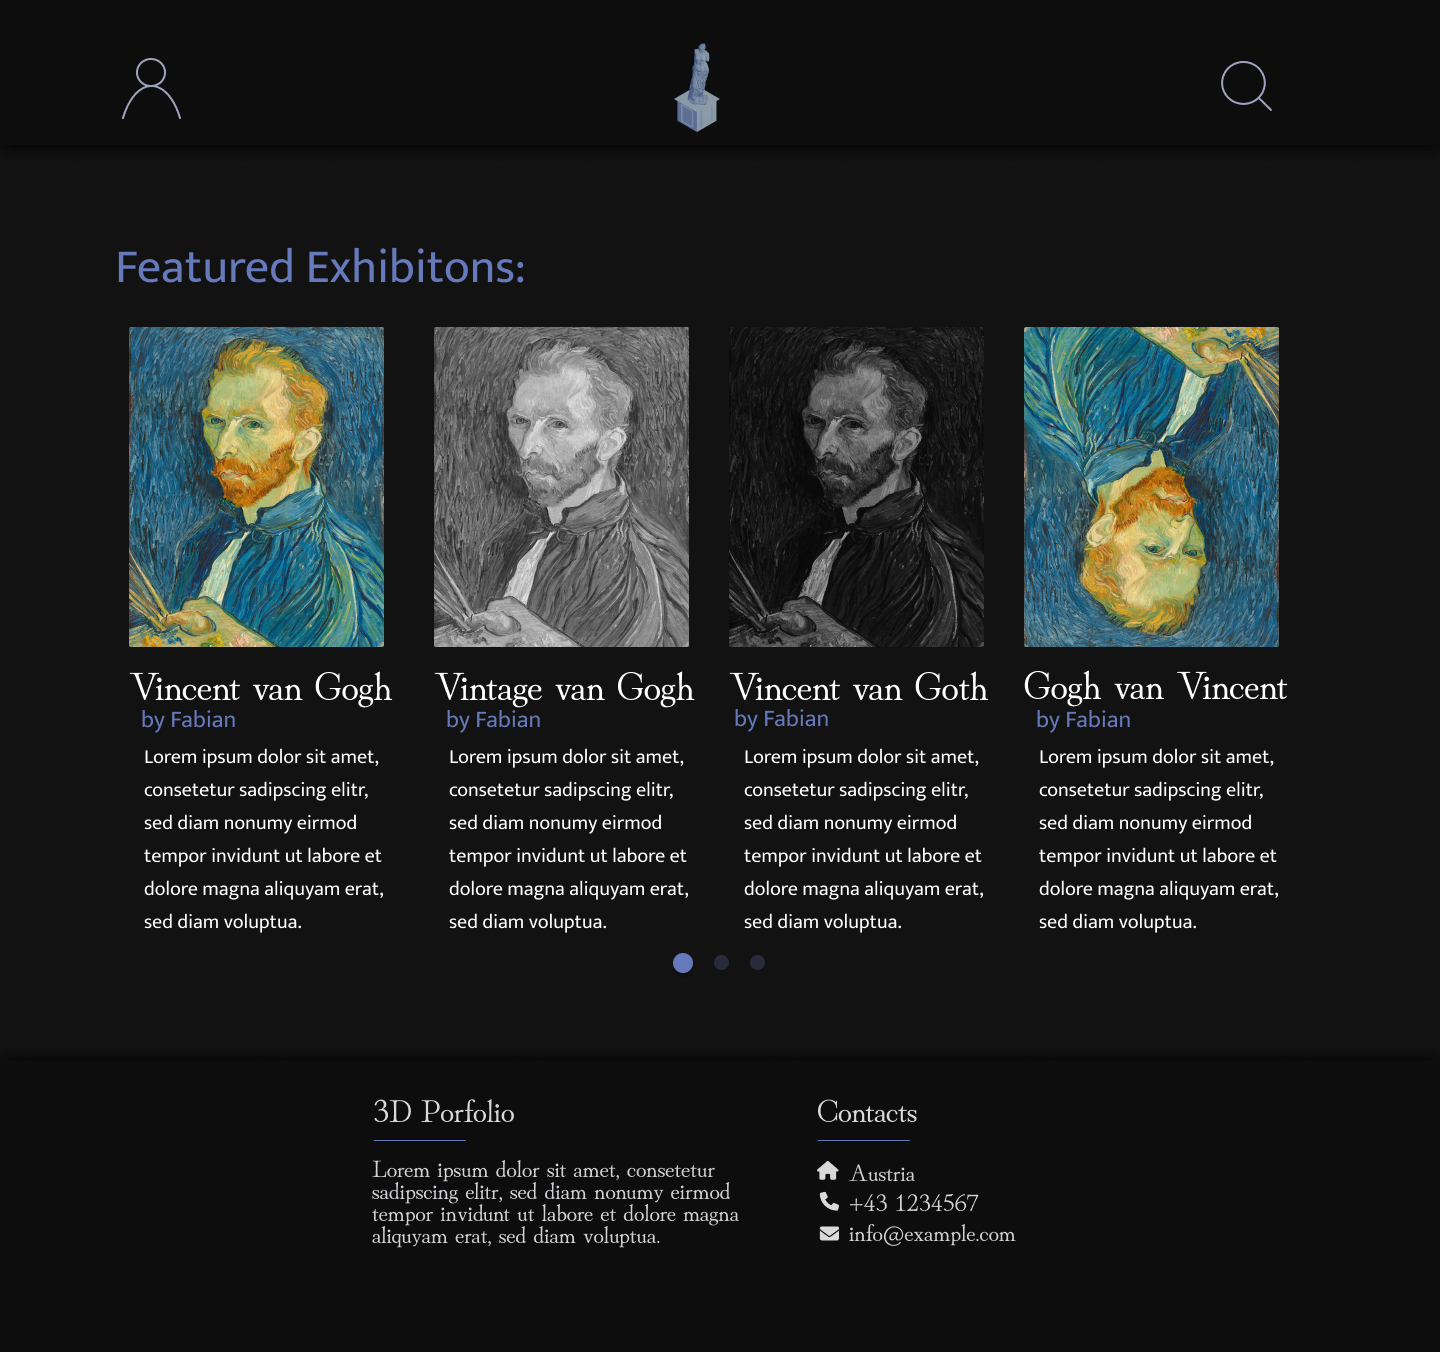
\includegraphics[scale=0.3]{pics/DesignKonzept1_2.png}
    \caption{Design Konzpet 1 Page 2}
    \label{fig:impl:knuth}
\end{figure}

\begin{figure}
    \centering
    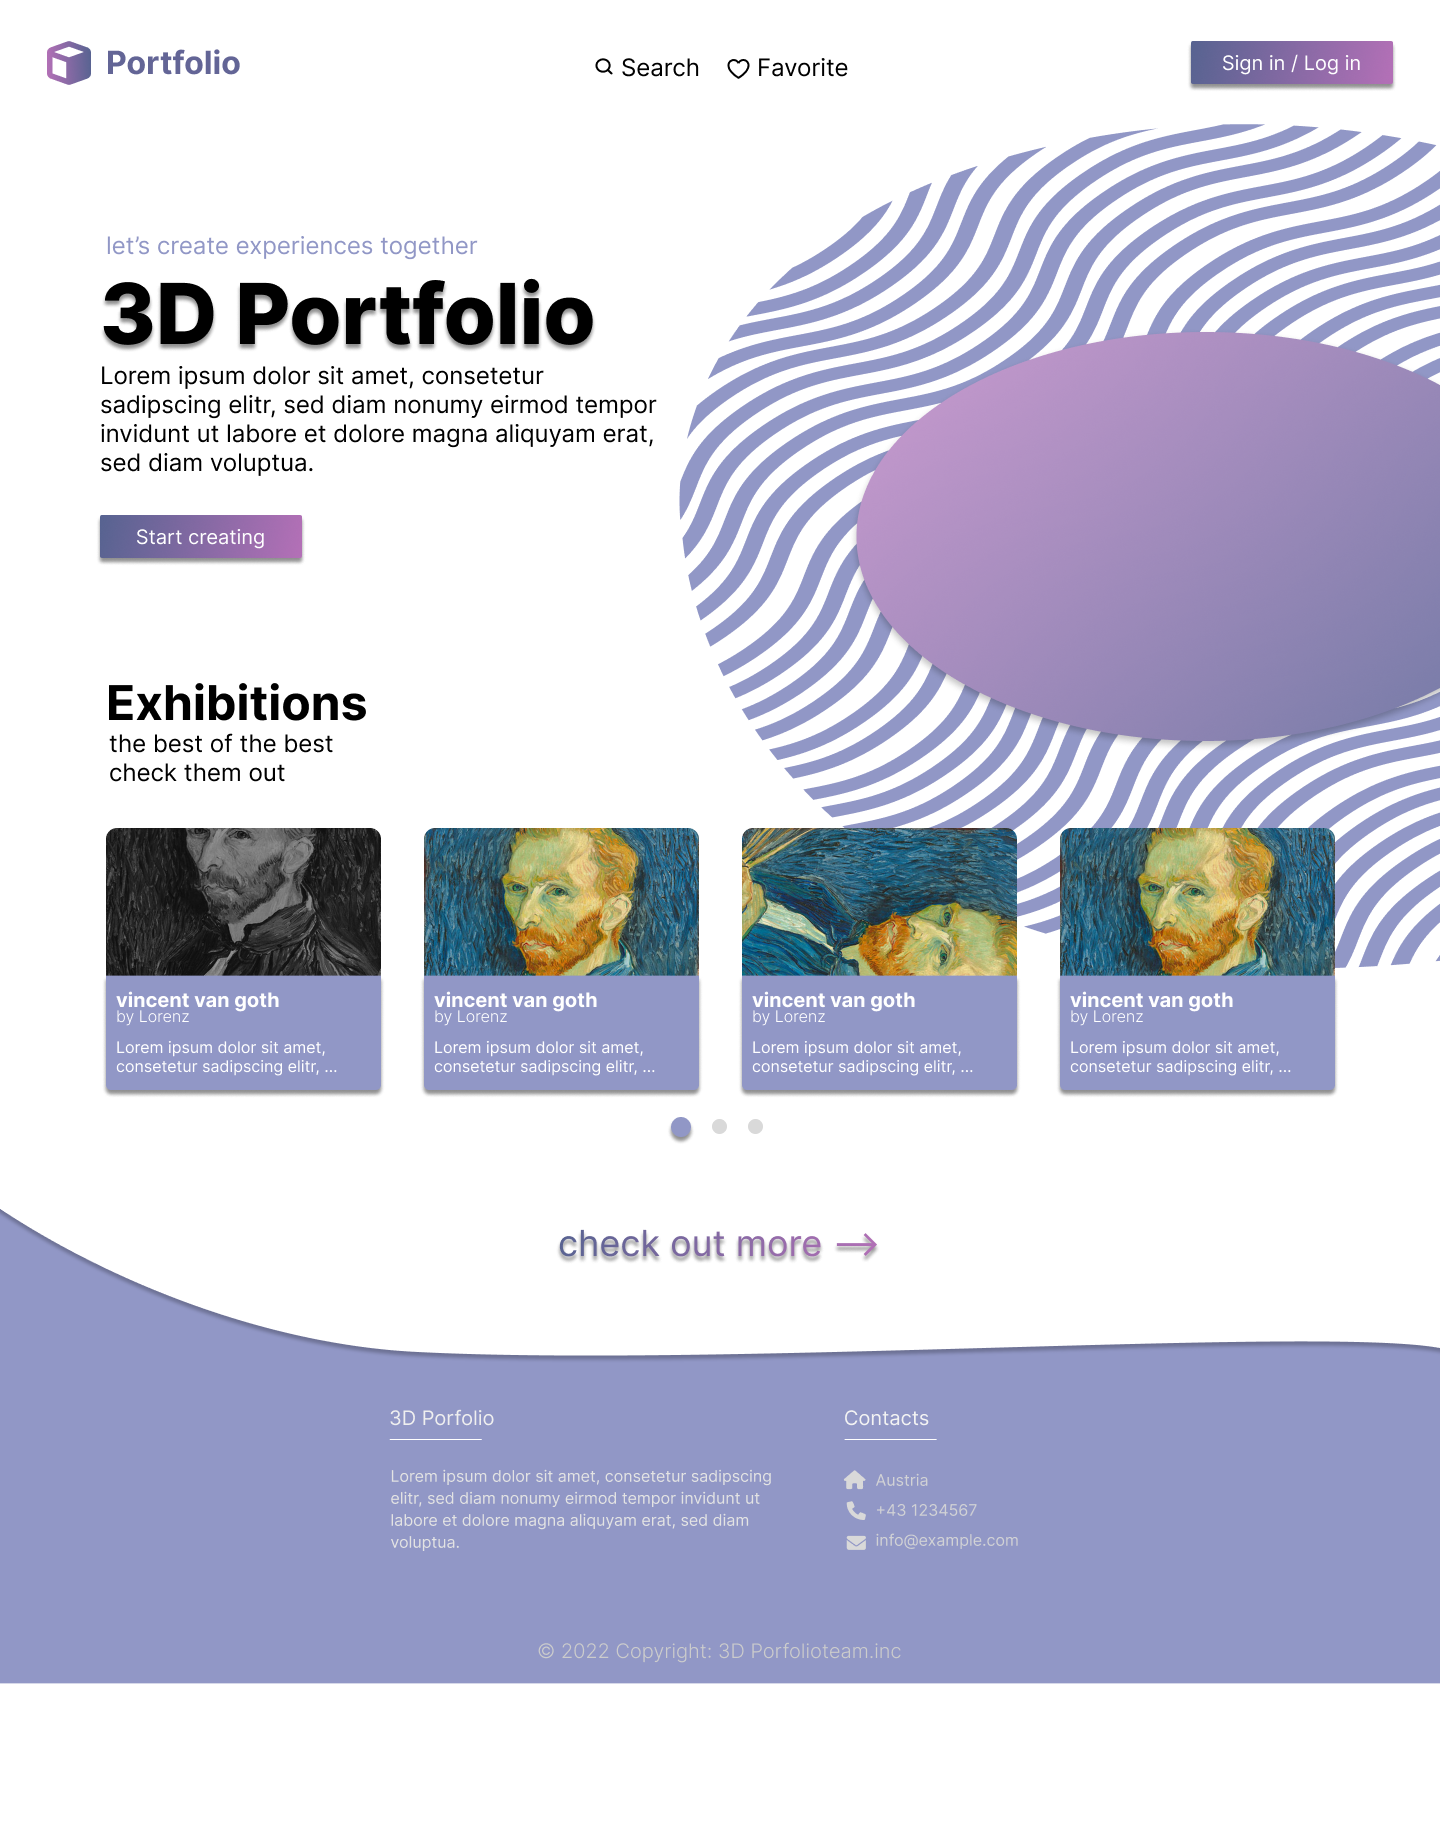
\includegraphics[scale=0.3]{pics/DesignKonzept2.png}
    \caption{Design Konzept 2}
    \label{fig:impl:knuth}
\end{figure}


\section{Umsetzung der Landingpage [L]}
\label{landingpage implentation}
\setauthor{Litzlbauer Lorenz}

Der erste Entwicklungsschritt für die vollständige Single-Page-Application beginnt mit der Initialisierung der Landingpage. Aus Sicht der User-Experience war es uns wichtig, dass der*die neue Nutzer*in sofort den Verwendungszweck des Applikation begreift und dazu animiert wird, bei der Applikation mitzumachen. 

Die Entwicklung startete damit, dass die benötigten Technologien Angular, AngularThree, AngularMaterials und Bootstrap heruntergeladen wurden.

Dafür wurde der \emph{NPM} Node-Package-Manager verwendet.

\subsubsection{Angular installieren}\label{sec:AngularCLI}
Angular hat ein eigenes Tool, die Angular CLI (Command Line Interface), um Projekte zu erstellen und zu bearbeiten, sowie um Komponenten, Services und vordefinierte Codemodule hinzuzufügen.

\begin{lstlisting}[caption={{Terminalm - Angular aufsetzen, Installation der CLI, Configuration eines neuen Projektes, Starten des Projektes}},language=bash]
npm install -g @angular/cli 
ng new Gallery
? Would you like to add Angular routing? Yes
? Which stylesheet format would you like to use? SCSS   [ https://sass-lang.com/documentation/syntax#scss ]
cd Gallery
ng serve -o
\end{lstlisting}

In der ersten Codezeile wird das Angular-CLI-Tool global von NPM installiert.
Danach wird mit dem Befehl \emph{ng new} mit dem CLI-Tool ein neues Angular Projekt erstellt. Anschließend gibt es mehrere Konfigurationsauswahlmöglichkeiten. Für dieses Projekt wurde das Routing (siehe \ref{sec:Routing}) aktiviert und als Stylesheet-Formatierung SCSS ausgewählt. Daraufhin wurde in das (Projekt-) Verzeichnis Gallery gewechselt und dort mit dem Befehl \emph{ng serve} ein Webpack-Server gestartet, welcher den vorgenerierten Code von dem neu erstellen Angular-Projekt zeigt (siehe in Abbildung \ref{fig:impl:angular-starting-page}). 

\begin{figure}
    \centering
    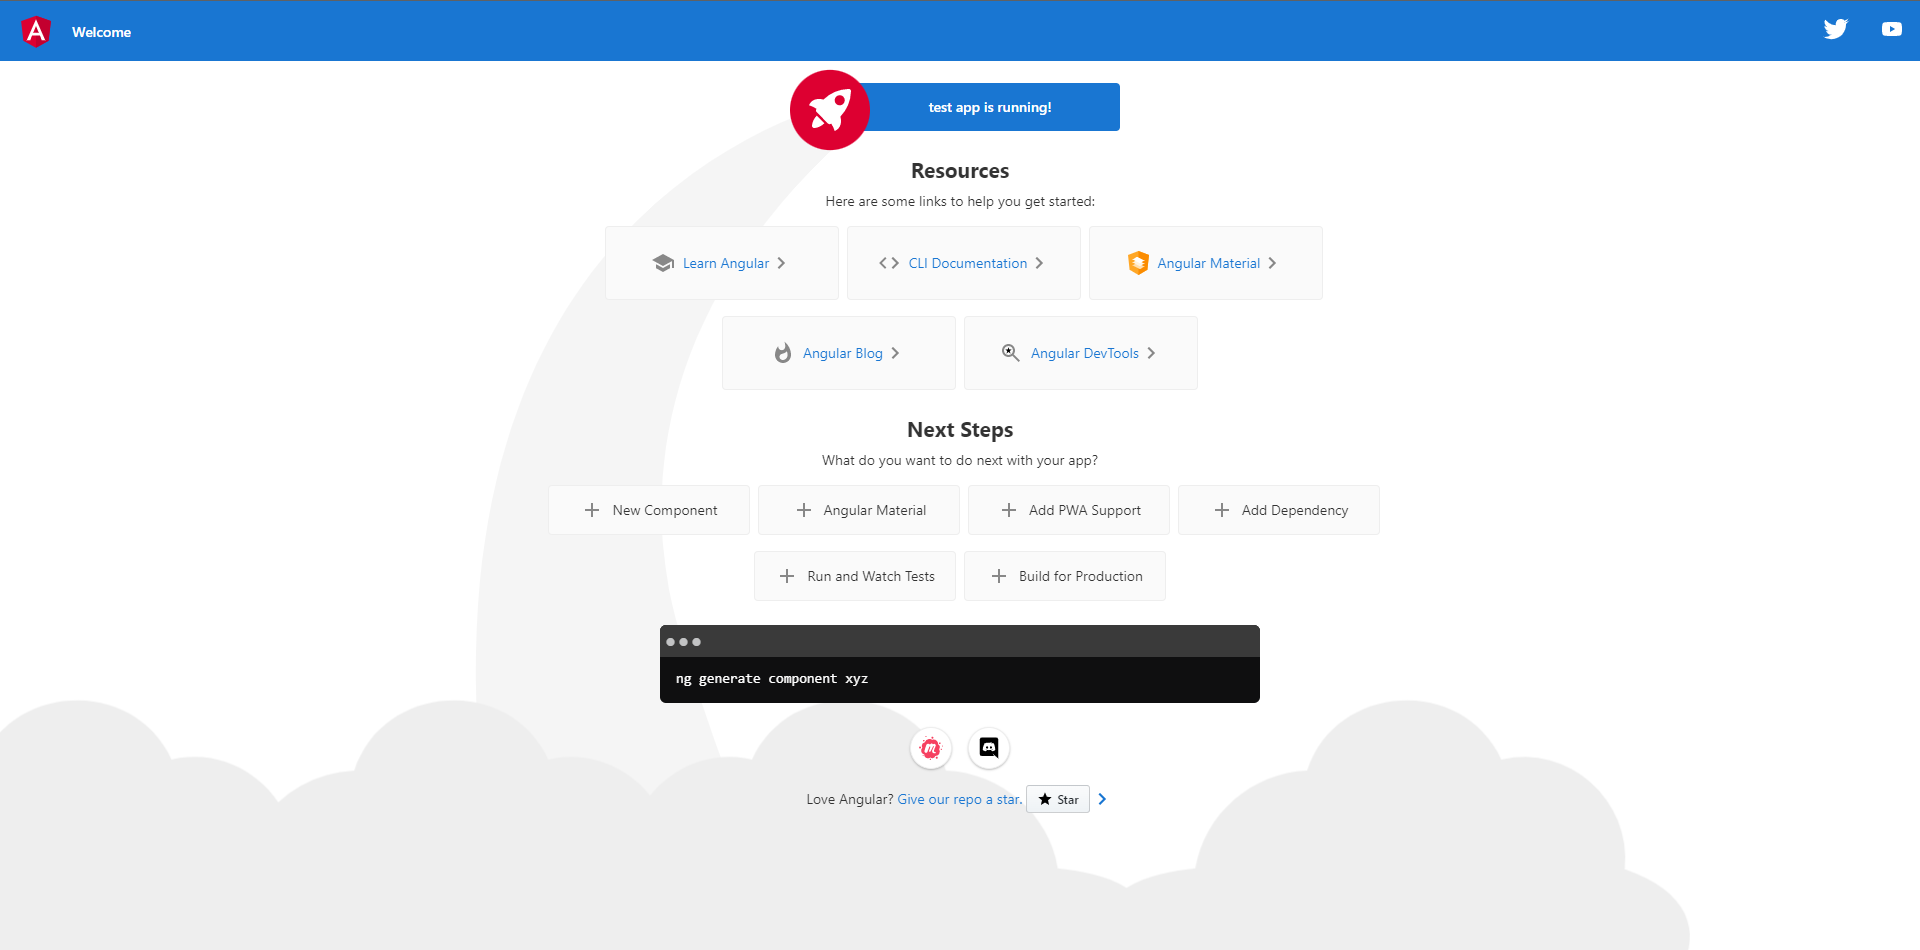
\includegraphics[scale=0.25]{pics/AngularStartingPage.png}
    \caption{Angular: Automatisch generierte Start-Webseite}
    \label{fig:impl:angular-starting-page}
\end{figure}

\paragraph{Globale oder lokale Module}
Bei einer lokalen Installation werden die installierten Module in einem Node-Modul-Computerordner lokal im Projekt abgespeichert, während alle globalen Installationen in einem einzigen Computerordner abhängig vom Computersystem gespeichert werden.

Generell kann man bei NPM-Modulen zwischen lokalen und globalen Installationen unterscheiden. Grundsätzlich wird eine lokale Installation empfohlen, referenzieren mehrere Projekte auf ein globales Modul, kann es dazu kommen, dass bei einer Aktualisierung des globalen Modules verschiedene Projekte beschädigt werden.
Das kommt daher, dass die darauf referenzierenden Projekte wegen ihrer Funktionalität anders auf die Veränderung des Modules reagieren.
CLI-Module haben eine Berechtigung dafür, global installiert zu werden. Denn CLI-Module sind abgekapselte Softwarelösungen, auf die kein anderes Projekt referenziert. Sie können auch lokal installiert werden und mit dem Befehl \emph{npx} nur im Projektordner ausgeführt werden.\cite{npmlocalorglobal}

\subsubsection{Installation der UI-Frameworks}

Nach der Installation von Angular wurden die UI-Frameworks \emph{Angular Material} und \emph{Bootstrap} installiert. 

\emph{Angular Material} konnte mithilfe des Befehls  \ref{lst:impl:installationAngularMaterials} mittels der Angular CLI in das Angularprojekt eingebunden werden.

\begin{lstlisting}[caption={{Terminal - Angular Material Installation}},language=bash,label=lst:impl:installationAngularMaterials]
    ng add @angular/material
\end{lstlisting}

Bootstrap wurde mithilfe des Befehls \ref{lst:impl:installationBootstrap} von NPM installiert.
Anschließend muss noch eine Verknüpfung zwischen Bootstrap und Angular hergestellt werden. Dafür musste in der Angular-Konfigurationsdatei \emph{angular.json} die Bootstrap Scss-Liberay eingebunden werden. Das wird in dem Code Beispiel \ref{lst:impl:BootstraptConfig} veranschaulicht.

\begin{lstlisting}[caption={{Terminal - Bootstrap Installation}},language=bash,label=lst:impl:installationBootstrap]
    npm i bootstrap
\end{lstlisting}

\begin{lstlisting}[caption={{angular.json - Bootstrap Angular Verknüpfung}},label=lst:impl:BootstraptConfig]
    {
        ...,
        "projects": {
            "Gallery": {
                ...,
                "architect": {
                    "build": {
                        ...,
                        "options": {
                            ...,
                            "styles": [
                                ...,
                                "node_modules/bootstrap/scss/bootstrap.scss"
                            ]
                        }
                    }
                }
            }
        },
        ...
    }
    
\end{lstlisting}


\subsubsection{Installation von Three.js}
Nach der Installation der UI-Libraries wurde Three.js installiert. 

\begin{lstlisting}
    npm install three
    npm i @types/three
\end{lstlisting}

\subsection{Komponenten [M]}
\label{components}
\setauthor{Fabian Maar}
Der nächste Schritt der Entwicklung ist das Erstellen der Komponenten und das Festlegen ihrer Struktur. Eine Komponente kann ebenfalls über die Angular CLI erstellt werden:

\begin{lstlisting}[caption={{Terminal - Component erstellen}},language=bash,label=lst:impl:addComponent]
    ng generate component home-page
\end{lstlisting}

\subsubsection{Allgemein}
Angular Komponenten lassen sich mit einem eigenen HTML-Selektor (z.B. <my-component>) ansprechen und in die Benutzeroberfläche einbinden. Komponenten besitzen viele Features, die den Entwicklungsprozess, Wartung des Codes und Fehlersuche erleichtern können:

\begin{itemize}
    \item Trennung von Logik und Design
    \item Skalierbarkeit der Applikation
    \item Data-Binding
    \item Hierarchie
    \item Lesbarkeit/Übersichtlichkeit
\end{itemize}

\subsubsection{Aufbau}
Um die Logik strikt von der Benutzeroberfläche zu trennen, werden die Dateien und der Code innerhalb einer Komponente strukturiert und separiert. Eine Komponente besteht somit aus: 

\begin{itemize}
    \item einem HTML-Template, dass die Benutzeroberfläche darstellt
    \item einer TypeScript-Klasse, die die Logik und Funktionalitäten der Komponente beinhaltet
    \item einem Stylesheet, dass das Aussehen der Benutzeroberfläche beeinflusst
    \item einer TypeScript-Testklasse, um individuell Komponenten zu testen 
\end{itemize}

\cite{AngularComponentOverview}

\subsubsection{Skalierung}
Die Skalierung beschreibt, wie gut eine Applikation mit Erweiterungen und ihrem Wachstum umgeht. Dabei wird geschaut, wie leicht sich zusätzliche Änderungen und Features implementieren lassen oder wie sich die Performanz der Anwendung bei zunehmender Größe verhält. Angular unterstützt dies durch einige Features:

TypeScript hilft durch seine Code-Syntax, auch bei großen Applikationen schnell Fehler zu erkennen. 

Durch die Angular CLI kann schnell und einfach ein Grundgerüst für die Entwicklung erstellt werden. Weiteres können Komponenten, Services und andere Angular Funktionen in jedem Entwicklungsstadium problemlos hinzugefügt werden, ohne dass der bestehende Code beeinflusst wird (siehe \ref{sec:AngularCLI}).

Angular stellt zudem Libraries wie Angular Materials oder das \emph{Component Development Kit (CDK)} zur Verfügung. Dadurch können problemlos vorgefertigte Angular Komponenten und Designs zu einer Applikation hinzugefügt werden.

\cite{AngularScaling}

\subsubsection{Hierarchie}
Die Hierarchie von Angular Komponenten lässt sich wie folgt in einer Baumstruktur abbilden:

\begin{figure}
    \centering
    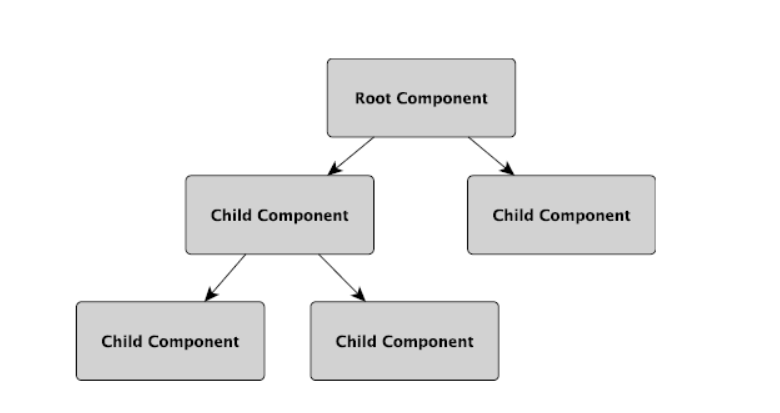
\includegraphics[scale=0.6]{pics/hierarchy.PNG}
    \caption{Component-Hierarchy \cite{AngularBuch}}
    \label{fig:tech:front:component-hierarchy}
  \end{figure}
Die Hauptkomponente ist der \emph{Root-Component}. Von ihr aus lassen sich weitere \emph{Child-Components} ineinander verschachteln. Diese Verschachtelung ist der Grund, warum die Anwendung in viele einzelne Teile ausgelagert werden kann. Außerdem können Komponenten durch das \emph{Data-Binding} untereinander Daten austauschen. \cite{AngularComponentsHierarche} \cite{AngularBuch}

\subsubsection{Data-Binding }
\label{data-binding}

\emph{Data-Binding} ist eine Methode, Daten zwischen der Logik und der Benutzeroberfläche auszutauschen. Dabei bleibt die Website ohne Refresh immer aktuell. Das Binden von Daten kann direkt am DOM (siehe \ref{txt:glos:DOM}) erfolgen, wofür es eine eigene Code-Syntax gibt. Beim Data-Binding wird zwischen  verschiedenen Kategorien unterschieden \cite{AngularBuch} \cite{BindingSyntax}:  
    

\paragraph{Interpolation}
Bei der \emph{Interpolation} werden Daten innerhalb einer Komponente von der Datenquelle in das HTML-Template eingefügt. Die Anzeige wird auch automatisch aktualisiert, wenn sich Daten im Hintergrund ändern. \cite{BindingSyntax}

\begin{lstlisting}[caption={{Beispiel für Interpolation in der 3D-Gallery}},language=HTML,label=lst:impl:interpolation]
    <div>
    <p class="text-center py-2">{{exhibit.title}}</p>
    </div>
\end{lstlisting}

\paragraph{Property-Bindings}
Beim \emph{Property-Binding} werden Daten direkt an ein DOM-Element übermittelt und ausgewertet. Somit werden die Attribute, das Aussehen und die Funktionen der jeweiligen DOM-Elemente dynamisch beeinflusst und automatisch bei Datenänderung aktualisiert. \cite{AngularPropertyBinding}
\begin{lstlisting}[caption={{Beispiel für Property-Bindings in der 3D-Gallery}},language=HTML,label=lst:impl:property-binding]
    <img [src]="user?.icon_url ?? 'assets/image/profile-photo.jpg'">
\end{lstlisting}

\paragraph{Event-Bindings}
Um auf Eingaben und Interaktionen von Benutzer*innen zu reagieren, werden Event-Bindings verwendet. Dabei werden die Daten vom HTML-Template zur TypeScript-Klasse übertragen und können dort genutzt werden. Sie sind also das Gegenstück zu den Property-Bindings. \cite{AngularEventBinding}
\begin{lstlisting}[caption={{Beispiel für Event-Bindings in der 3D-Gallery}},language=HTML,label=lst:impl:event-binding]
    <button(click)="delete()">
      <mat-icon>close</mat-icon>
    </button>
\end{lstlisting}

\paragraph{Two-Way-Bindings}
Das \emph{To-Way-Binding} benutzt beide Varianten, Property- und Event-Binding, um Daten auszutauschen. Hierbei ist es möglich, die Daten sowohl von der TypeScript-Klasse zum DOM-Element zu übertragen und umgekehrt. \cite{AngularTwoWayBinding}
\begin{lstlisting}[caption={{Beispiel für Two-Way-Bindings \cite{AngularTwoWayBinding}}},language=HTML,label=lst:impl:two-way-bindings]
    <app-sizer [(size)]="fontSizePx"></app-sizer>
\end{lstlisting}
In den folgenden Kapitel werden die Komponenten und ihre Funktionalitäten näher beschrieben. 

\subsection{Routing [M]}\label{sec:Routing}
\emph{Routing} ist das Konzept einer Single-Page-Applikation, wodurch die Seite niemals neu geladen werden muss und alle Daten beim Navigieren beibehalten werden können. Beim Routing werden dabei bestimmte Komponenten angezeigt, abhängig von der aktuellen URL. Dabei kann durch die Applikation navigiert werden, was durch den sogenannten \emph{Router} realisiert wird.  Um das Routing überhaupt verwenden zu können, müssen die Pfade zu den zugehörigen Komponenten initialisiert werden. Dies geschieht in einem \emph{ngModule}, wo alle initialisierten Routen über das \emph{RouterModule} importiert werden. Um die Funktionalitäten und Routen für alle Komponenten verwenden zu können, muss dieses \emph{RouterModule}ebenfalls exportiert werden. Der Code zeigt dies anhand der 3D-Gallerie-Anwendung: \cite{AngularBuch}
\begin{lstlisting}[caption={Routing in der 3D-Gallery},language=TypeScript,label=lst:impl:routing]
const routes: Routes = [
  {path: '', component:HomePageComponent},
  {path: 'home', component:HomePageComponent},
  {path: 'log-signin', component:LogSigninPageComponent},
  {path: 'search', component:SearchPageComponent},
  {path: 'profile', component:ProfilePageComponent},
  {path: 'create', component:CreateExhibitionPageComponent},
  {path: 'signup', component:SignupPageComponent},
  {path: 'room/:id', component:RoomPageComponent},
  {path: '**', redirectTo: 'home'}
  ];
  @NgModule({
    declarations: [],
    imports: [ CommonModule, RouterModule.forRoot(routes) ],
    exports: [ RouterModule ]
  })

\end{lstlisting}
Hierbei steht der Pfad ‘**’ für alle ungültigen URLs wodurch der*die Benutzer*in auf die Landingpage geleitet wird.

Ebenfalls wird das Routing genutzt um das Navigieren durch die Navbar (siehe fertige Landingpage \ref{Finished Landingpage}) zu ermöglichen. Hierbei wird ein deklarierter Pfad direkt mit einem HTML-Element, über das Attribut \emph{routerLink}, verbunden. Falls sich der*die Benutzer*in auf auf dem momentanen Pfad des \emph{routerLinks} befindet, wird das Attribut \emph{routerLinkActive} aktiv. Dadurch kann dem*der Benutzer*in ein bestimmtes visuelles Feedback geliefert werden.  (siehe Code \ref{lst:impl:routerLink})

\begin{lstlisting}[caption={Routing über einen routerLink},language=HTML,label=lst:impl:routerLink]
    
          <a class="navbar-brand"
             routerLink="/home" routerLinkActive="link-activated"><mat-icon>home</mat-icon>Home</a>
          <a class="navbar-brand"
             routerLink="/search" routerLinkActive="link-activated"><mat-icon>search</mat-icon>Search</a>
          <a class="navbar-brand" *ngIf="this.auth.isLoggedIn()"
             routerLink="/profile" routerLinkActive="link-activated"><mat-icon>person</mat-icon>Profile</a>
       
\end{lstlisting}

\subsubsection{Routingparameter}
\label{Routingparameter}
Um Routen dynamisch zu deklarieren, werden sogenannte Routenparameter benötigt. Hierbei beginnt der dynamische Teil einer Route mit einem Doppelpunkt. 


\begin{lstlisting}[caption={Routingparamter in der 3D-Gallery},language=TypeScript,label=lst:impl:routingparameter]
    const routes: Routes = [
      {path: 'room/:id', component:RoomPageComponent},
      ];    
\end{lstlisting}

Um den aktuellen Zustand der URL auszulesen, muss der Router im Konstruktor injiziert werden. Anschließend kann der Parameter wie folgt ausgelesen und als Wert einer Variable zugewiesen werden:

\begin{itemize}
    \item Dies geschieht entweder über die \emph{Snapshot-Methode}, die den momentanen Zustand der URL ausliest 
    \begin{lstlisting}[caption={Snapshot der URL abfragen},language=TypeScript,label=lst:impl:routingsnapshot]
        this.id = this.route.snapshot.paramMap.get('id');
    \end{lstlisting}
    \item oder, wie auch im Projekt der 3D-Gallery umgesetzt, über das \emph{Observable-Pattern} (siehe \ref{txt:glos:observerDesignPattern}) auf den Router \ref{subscriben}, um auf ständige Änderungen im Pfad zu reagieren:
    \begin{lstlisting}[caption={Die URL subscriben},language=TypeScript,label=lst:impl:urlsubscription]
        this.sub = this.route.params.subscribe(params => {
            this.id = +params['id'];
          })
    \end{lstlisting}
\end{itemize}
\cite{AngularBuch}
\section{Angular Services [M]}
Um eine Schnittstelle zwischen dem Backend und dem Frontend herzustellen, werden Angular Services verwendet.

\subsection{Allgemein}
Ein Service in Angular ist eine TypeScript-Klasse, die verwendet wird, um Logik auszulagern, die von der gesamten Applikation verwendet werden kann. Services werden meist dann erstellt, wenn eine einfache Logik oft von verschiedenen Komponenten benötigt wird. Um die globale Verwendung zu realisieren, wird das Konzept der Dependency Injection verwendet. \cite{AngularBuch} \cite{AngularArchitectureService}

\subsection{Dependency Injection}
In Angular ist es möglich, einen Service in eine beliebige Komponente zu injizieren. Das bedeutet, ein Service wird anhand von @Injectable() definiert und dadurch kann dieser von anderen Komponenten verwendet werden \cite{AngularBuch}:

\begin{lstlisting}[caption={Eine Klasse Injectable machen},  language=TypeScript,label=lst:impl:injectable]   
    
 @Injectable({
 providedIn: 'root'
 })
  export class GalleryService{
    ..
  }
   
\end{lstlisting}

Auch wird ein Provider mit angegeben. Dieser sorgt dafür, dass sich Services entweder nur in spezifische Komponenten injizieren lassen oder sich wie hier auf root-level, also überall injizieren lassen. \cite{AngularBuch}

Ein Service wird zur Verwendung im Konstruktor einer Komponente initialisiert (Constructor Injection): 

\begin{lstlisting}[caption={Constructor Injection},  language=TypeScript,label=lst:impl:concstructorinjection]   
    constructor(private gs: GalleryService) { }
\end{lstlisting}
Anschließend können die Methoden und Daten eines Service ganz normal verwendet werden

\subsection{HTTP Module}
Um mit dem Backend über das HTTP-Protokoll kommunizieren zu können, wird eine HTTP-API //TODO REFERENZ API namens HttpClient verwendet. Zunächst muss das HttpClientModule im ngModule importiert werden, um den HttpClient als Dependency zu injizieren. Injiziert wird er über den Konstruktor in einem Service. Um eine Transaktion am Frontend durchzuführen, werden Observables verwendet. Dies ermöglicht den einzelnen Komponenten, die einen Service mit HTTP-Abfragen injiziert haben, diese Abfragen mittels einem Subscribe zu nutzen. Eine HTTP-Abfrage mit dem HTTP-Client wird wie folgt aufgerufen \cite{AngularBuch} \cite{AngularHTTPClient}:

\begin{lstlisting}[caption={HttpClient Abfragen},  language=TypeScript,label=lst:impl:httpclientrequests]   
    URL = "http://localhost:8080/api/"

    getAllRooms(): Observable<Room[]>{
        return this.httpClient.get<Room[]>(`${this.URL}rooms/allRoomPositions`);
      }
    
\end{lstlisting}

Wie anhand des oberen Code-Beispiels erkennbar ist wird hier das Room-Interface benutzt.

\subsection{Interface [M]}

Interfaces werden verwendet, um typsicher ein Objekt zu strukturieren. Dabei wird, um Daten des Servers korrekt erhalten zu können, eine bestimmte Entität der Datenbank verglichen und durch die richtige Benennung und Datentyp im Frontend abgebildet. Üblicherweise exportiert man ein solches Datenobjekt, um es in der ganzen Anwendung zu verwenden. Folgendes Beispiel demonstriert dieses Konzept anhand des Exhibit-Interfaces \cite{AngularBuch}: 

\begin{lstlisting}[caption={Das Datenmodell eines Ausstelungsstückes},  language=TypeScript,label=lst:impl:httpclientrequests]   
  
export class Exhibit{
    id : number;
    url : string;
    data_type : string;
    title : string;
    description : string;
    alignment: string | undefined
    position: Position | undefined
    scale: number | undefined
  
    constructor(id: number, model_url: string, data_type: string, title: string, desc: string, alignment: string | undefined, position: Position | undefined, scale: number | undefined) {
      this.id = id;
      this.url = model_url;
      this.data_type = data_type;
      this.title = title;
      this.description = desc;
      this.alignment = alignment
      this.position = position
      this.scale = scale
    }
}
\end{lstlisting}


\section{Web Gallery Prototype}
\subsection{Zusammenfassung [M]} 
\setauthor{Fabian Maar}
In diesem Abschnitt wird erklärt, auf welche Weise die 3D-Ausstellung in der Webapplikation realisiert wurde. Dabei wurde das Konzept des evolutionären Prototypings (siehe Prototyping \ref{ch::ongoing-prototyping}) für die Entwicklung verwendet. 

\subsection{Rendering [M]} 
Um 3D-Modelle, wie den Ausstellungsraum anzeigen zu können, wird der hochkomplexe Prozess des Renderings benötigt. Dabei wird das 3D-Modell zu einem realistischen 2D-Bild gerendert. 
\cite{AdobeRendering} \cite{Rendering3DModels}

\subsubsection{Der Prozess des Renderings}
Hinter dem Rendering stecken verschiedene Algorithmen, die ein solches 3D Modell anzeigen lassen. Verschiedene Werte und Daten werden zur Berechnung benötigt, welche die Qualität und die Geschwindigkeit des Prozesses unterschiedlich beeinflussen:

\begin{itemize}
    \item das 3D-Objekt und wie realistisch es dargestellt werden soll
    \item die Art des Renderns
    \item die Lichtquellen und die entstehenden Schatten; wird Behandel im Kapitel Lichtsetzung \ref{lichtsetzung}
    \item die Kameraposition und Renderbereich (Clipping)
    \item der Anti-aliasing Prozess
    \item die Art des Render-Algorithmuses
    \item weitere atmosphärische Effekte 
    
    
\end{itemize}
\cite{Rendering3DModels}

\subsubsection{3D-Modelle}
3D-Modelle besitzen verschiedene Eigenschaften, wie zum Beispiel ihre Textur, Farbe oder ihre Fähigkeit Licht zu reflektieren, die beim Rendern berücksichtigt werden müssen. Die 3D-Daten des Modells werden ermittelt und dabei in Pixelinformationen umgewandelt. Diese werden durch die Ermittlung der Koordinaten des Objektes an bestimmten Positionen abgebildet. \cite{Rendering3DModels}

\subsubsection{Arten des Renderns}
Beim Rendern wird zwischen folgenden Arten unterscheiden:

\begin{itemize}
    \item Offline-Rendering - Das Offline-Rendering rendert über einen längeren Zeitraum in hoher und realistischer Qualität. Diese Art kommt zum Beispiel bei Filmen zum Einsatz. 
    \item Echtzeit-Rendering - Beim Echtzeit-Rendering wird ein 3D-Modell in kürzester Zeit gerendert. Diese Art kommt zum Beispiel bei Videospielen oder im 3D-Gallery zum Einsatz. Hierbei werden meist 24 Bilder pro Sekunde gerendert, um Bewegungen flüssig wahrzunehmen. 
\end{itemize}
\cite{RenderArten}

\subsubsection{Clipping}
\label{clipping}
Beim Clipping werden Ebenen zur Begrenzung des Bereichs, den es zu rendern gilt, erstellt. Diese Ebenen werden durch die Weltkoordinaten positioniert. Die seitlichen sowie die unteren und oberen Clipping-Ebenen werden durch die Kameraposition und die Fensterposition definiert. Auch gibt es das Far- und Near-Clipping, wodurch zum einen die Tiefe des 3D-Modells begrenzt wird. Zum anderen werden unerwünschte Objekte, die im Hintergrund liegen, ebenfalls nicht gerendert. \cite{Rendering3DModels}


\subsubsection{Anti-Aliasing}
Beim Anti-Aliasing Prozess wird versucht, den auftretenden Aliasing-Effekt zu reduzieren und zu entfernen. Der Aliasing-Effekt tritt auf, wenn die Pixel zu grob für feine Strukturen und Muster sind. Der Effekt ist besonders stark, wenn diese Muster nicht senkrecht sind. Dieser Aliasing-Effekt wirkt sich auf das 3-Modell aus, in dem Zacken an Polygon-Kanten entstehen, ein Moiré-Effekt auftritt ( siehe Abbildung \ref{fig:impl:MoireEffekt}) Verweis oder generell unerwünschte Muster auftreten.\cite{Rendering3DModels} 
\begin{figure}
    \centering
    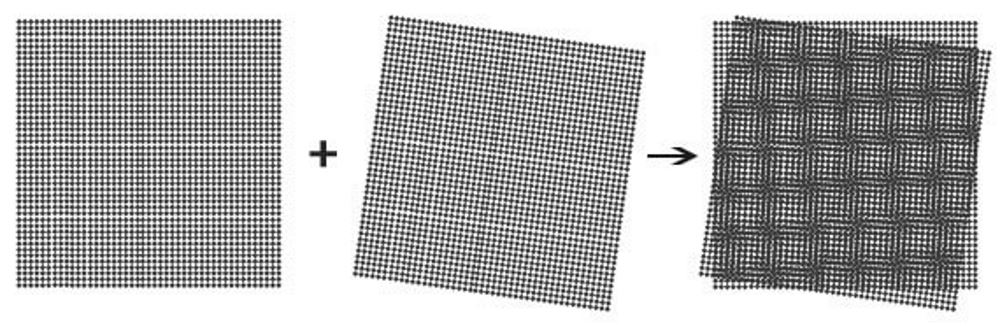
\includegraphics[scale=0.3]{pics/moire-effekt.jpg}
    \caption{Der Moire-Effekt visualisiert \cite{MoireEffekt}}
    \label{fig:impl:MoireEffekt}
\end{figure}

\begin{figure}
    \centering
    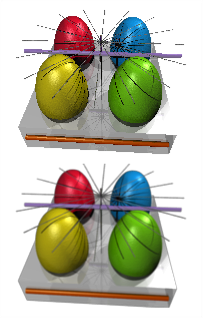
\includegraphics[scale=0.7]{pics/anti-aliasing.png}
    \caption{Rendering mit und ohne Anti-Aliasing \cite{AntiAliasing}}
    \label{fig:impl:anti-aliasing}
\end{figure}

\subsubsection{Verschiedene Render-Algorithmen [M]}
\subsubsection{Rasterization}
Über den Bildschirm wird ein Raster aus meistens Dreiecken gespannt, da diese am einfachsten zu berechnen sind. In den Ecken der Dreiecke, auch genannt Scheitelpunkte, sind die Informationen enthalten, die zur Darstellung eines 3D-Objektes in 2D benötigt werden. Dieser Prozess wird für Echtzeit-Rendering genutzt. Er ist zwar rechenintensiv, jedoch nicht so intensiv wie beim Ray-Tracing. \cite{RayTracingRasterization}

\subsubsection{Wire-Frame}
Bei einem Wire-Frame wird ein 3D-Modell erstellt, in dem der Algorithmus versucht, lineare Merkmale wie Kanten oder Konturlinien zu verfolgen. Dabei werden auch verdeckte oder nicht-sichtbare Teile inkludiert. 
\cite{Rendering3DModels} 

\subsubsection{Visible Line}
Dieser Vorgang funktioniert ähnlich wie ein Wire-Frame, nur dass hierbei nur Linien gerendert werden, die tatsächlich von der Kamera sichtbar sind. Dieser sichtbare Bereich wird auch Visible Surface genannt. 
\cite{Rendering3DModels} 

\subsubsection{Raycasting}
\label{impl:rend:raycasting}
Beim Raycasting wird ermittelt, welches 3D-Objekt zuerst von einem Ray getroffen wird. Ein Ray ist ein Strahl, der von der Position der Kamera ausgeht. Für jedes Pixel wird ein Ray durch den dreidimensionalen Raum geschickt. Dadurch können die Schnittpunkte der Objekte und der Rays ermittelt werden. Dabei werden alle Objekte mit einem sichtbaren Schnittpunkt angezeigt und die Fläche normal dazu bestimmt die Schattierung. Dieser Prozess wird im Kapitel \ref{impl:int:raycasting} näher erklärt und angewandt.
\cite{Rendering3DModels} 

\subsubsection{Ray-Tracing}
Der Ray-Tracing Prozess funktioniert ähnlich wie der Prozess des Raycastings. Beim Ray-Tracing werden jedoch auch verschiedene Oberflächen und Lichtquellen berücksichtigt. Dies funktioniert, indem ein Ray vom Algorithmus mitverfolgt wird. Dabei ist es möglich, zu erkennen ob ein Ray:
\begin{itemize}
    \item durch eine lichtdurchlässige Oberfläche durchdringt
    \item von einem reflektierenden Objekt reflektiert wird
    \item oder ob ein Objekt von einer Lichtquelle getroffen wird und einen Schatten wirft
\end{itemize}
\cite{RayTracingRasterization}

\begin{figure} [h]
    \centering
    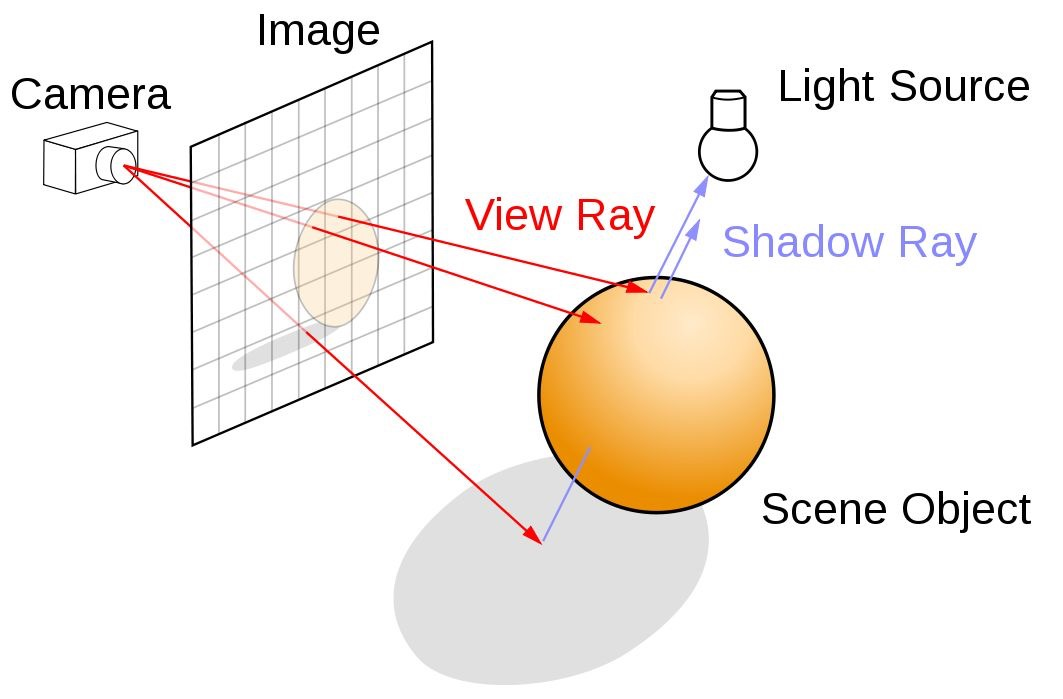
\includegraphics[scale=0.3]{pics/ray-tracing.jpg}
    \caption{Vorgang des Ray-Tracing \cite{RayTracingRasterization}}
    \label{fig:impl:ray-tracing}
\end{figure}


\subsubsection{Rendering in Three.js}
Für das Rendern der 3D-Gallery wird der in Three.js inkludierte Renderer von WebGL (siehe ThreeJS \ref{ch::webgl}) Referenz verwendet. Um das gerenderte 3D-Objekt in das DOM (siehe DOM \ref{txt:glos:API}) zu integrieren, wird das HTML-Element <canvas> verwendet. \cite{ThreejsWebGLRenderer}

\begin{lstlisting}[caption={Canvas-Element in HTML},language=HTML,label=lst:impl:canvas]
    <canvas #threeCanvas style="width: 100%;  height: 100%" (window:resize)="onResize($event)"></canvas>
\end{lstlisting}
Dabei wird dieses DOM-Element als Angular-View-Child initialisiert. Dadurch können Änderungen am Dom erkannt und das betroffene Element neu definiert werden. \cite{AngularViewChild}
\begin{lstlisting}[caption={Canvas als View-Child initialisieren},language=TypeScript,label=lst:impl:viewchild]
    @ViewChild('threeCanvas') threeCanvas!: ElementRef;
\end{lstlisting}
Anschließend wird ein neuer WebGLRenderer angelegt, dem der Canvas zugewiesen wird. Falls noch kein Canvas besteht, wird automatisch ein neuer erstellt. \cite{ThreejsWebGLRenderer}
\begin{lstlisting}[caption={WebGlRenderer anlegen},language=TypeScript,label=lst:impl:WebGlRenderer]
    this.renderer = new THREE.WebGLRenderer({
        canvas: this.threeCanvas.nativeElement
      });
\end{lstlisting}
Um die Render-Funktion des Renderers als Echtzeit-Rendering anzuwenden, wird eine Render-Schleife benutzt. Darin ist zum einen die Render-Funktion mit der Szene und der Kamera, die gerendert werden soll. In einer Szene befinden sich alle 3D-Objekte. Zum anderen befindet sich die Funktion requestAnimationFrame in der Schleife, wodurch die Szene jedes Mal neu gerendert wird, wenn der Bildschirm neu geladen wird. Dies geschieht üblicherweise 60-mal in der Sekunde. \cite{ThreejsCreateAScene}
\begin{lstlisting}[caption={Animations-Schleife},language=TypeScript,label=lst:impl:animationloop]
    animate = () => {
        requestAnimationFrame(this.animate);
        this.renderer.render(this.scene, this.camera!)
    }  
\end{lstlisting}
\subsection{Resizing [L]} 
\setauthor{Litzlbauer Lorenz}
https://www.omnicalculator.com/other/resolution-scale
https://discourse.threejs.org/t/render-half-size-then-upscale/13228

\subsection{Lichtsetzung}
\label{lichtsetzung}
Das Licht ist das 2. Wichtig, denn ohne würden die gerenderten Objekte im Dunklen stehen. Um dies zu ändern, wird eine Lichtquelle installiert, um einen bestimmten Bereich der Szene zu erhellen. Dabei können ebenfalls unterschiedliche Optionen konfiguriert werden, um die Szene so realistisch wie möglich aussehen zu lassen. Das Licht wird jedoch nicht nur von der Lichtquelle beeinflusst, sondern auch von dem Objekt, das beleuchtet wird. Material und Oberfläche eines Objektes reagieren unterschiedlich auf den Einfall des Lichtes, wodurch zum Beispiel die Lichtreflektion stärker ausfällt. Dieses Konzept wird auch Global Illumination genannt. Three.js bietet eine Vielzahl von Lichtarten und Quellen:

\begin{itemize}
    \item Das Standard-Licht, Light genannt, ist das Grundgerüst der anderen Lichttypen. Es kann die Farbe und Intensität des Lichtes individuell geändert werden. \cite{StandardLight}
    \item Die LightProbe ist eine alternative Methode, Licht zu erzeugen. Dabei wird nicht direkt von einer Quelle das Licht ausgestrahlt, sondern es speichert die Lichtinformation ab. Dabei wird erst beim Rendern der Lichteinfall durch die Daten der LightProbe ermittelt.  \cite{LightProbe}
    \item Das AmbientLight belichtet die gesamte Szene gleich, kann dabei jedoch keine Schatten werfen. \cite{AmbientLight}
    \item Das DirectionalLight wirft Licht parallel in eine bestimmte Richtung. Da es unendlich weit weg erscheint, wird es oft als Tages- oder Sonnenlicht verwendet. \cite{DirectionalLight}
    \item Das HemisphereLight wird über der Szene positioniert und besitzt eine Himmel- und Bodenfarbe mit Verlauf. Diese Lichtquelle kann keine Schatten werfen \cite{HemisphereLight}
    \item Das PointLight wirft Licht von einem Punkt in alle Richtungen. Es soll eine Glühbirne simulieren. Hierbei kann ebenfalls die Reichweite des Lichtes und ein Dimmeffekt bestimmt werden. \cite{PointLight}
    \item Das RectAreaLight strahlt Licht in Form eines Rechtecks aus. Damit können zum Beispiel Fenster simuliert werden \cite{ReactAreaLight}
    \item Das SpotLight wirft Licht in Form eines Kegel \cite{SpotLight}
\end{itemize}

Das Point Light wurde in der 3D-Ausstellung wie folgt angewandt:  
\begin{lstlisting}[caption={Lichtsetzung in der 3D-Ausstellung},language=TypeScript,label=lst:impl:pointlight]
    const bulbGeometry = new THREE.SphereGeometry(.02, 16, 8);
    const bulbLight = new THREE.PointLight( 0xffffff, 3, 1000, 2); 
    const bulbMat = new THREE.MeshStandardMaterial( {
          emissive: 0xffffff,
          emissiveIntensity: 1,
          color: 0x000000
        } );
        bulbLight.add( new THREE.Mesh( bulbGeometry, bulbMat ) );
        bulbLight.position.set( 0, 100, 0 );
        bulbLight.castShadow = true;
        this.scene.add( bulbLight );
\end{lstlisting}
Zunächst wurde ein Objekt angelegt, welches das Licht ausstrahlen soll. Anschließend wird die Lichtquelle und deren Material initialisiert. Um Schatten zu werfen, wird das Attribut .castShadow auf true gesetzt. 


\section{Fertige Landingpage [L][M]}
Die Landingpage (siehe Abbildung \ref{fig:impl:finishedLandingpage}) repräsentiert das Projekt, denn es ist das erste, was ein neuer Benutzer*in von der Webanwendung zu sehen bekommt. Es war wichtig, ein modernes Design dafür zu entwickeln.

Wichtige Punkte, die bei der Landingpage beachtet wurden, waren die Hierarchie der Elemente. Zuerst gab es eine Einleitung, um das Projekt zu erklären, danach kam ein großer Knopf, der dazu einlädt, das Produkt zu verwenden. Er verlinkt zu der Anmeldung. Danach kam eine Selektion aus den neuesten erstellten Ausstellungen, damit kann sich der User gleich ein Bild vom Projekt machen.

\begin{figure}
    \centering
    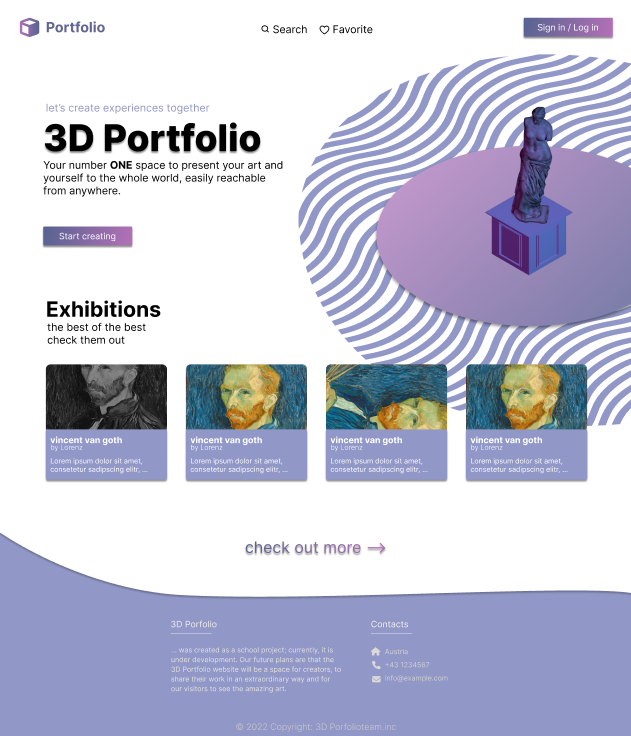
\includegraphics[scale=.5]{pics/startingpage.png}
    \caption{Landing Page}
    \label{fig:impl:finishedLandingpage}
\end{figure}

Um zwischen den verschiedenen Unterseiten der Webseite zu wechseln, wurde am oberen Bildschirmrand zusätzlich eine Navigationsleiste implementiert. Diese sogenannte Navbar besitzt je nach Unterseite verschiedene Designs. Dies ermöglicht ein angenehmes Navigieren auf jeder Seite (Siehe Routing \ref{lst:impl:routing}). Ebenfalls muss auch der Footer auf jeder Unterseite passend angezeigt werden. Um das Design der Navbar und Footer auf jeder Seite individuell zu gestalten, wird ein Service jeweils in die entsprechende Komponente injiziert. Dadurch können Konfigurationen am Design durch wenig Code und Redundanz vorgenommen werden. 

\subsection{Erledigte Userstories [L]}
\label{Finished Landingpage}
Bei der Fertigstellung der Landingpage wurden folgende Userstories vollendet: 
\begin{compactitem}
    \item Als erstmalige*r Besucher*in der Webseite möchte ich die benötigten Informationen über die Funktionen der Applikation verständlich erkennen können. Akzeptanzkriterien:
    Auf der Landingpage befinden sich:
    \begin{compactitem}
        \item Textstellen und Grafiken, die unser Projekt und die Funktionalitäten davon erklären
        \item Einen Call-to-Action(CTA)-Button, der den User*in dazu einlädt, seine eigene Ausstellung zu erstellen. Beim Betätigen wird der Benutzer, falls er schon eingeloggt ist, weitergeleitet zum Editor, sonst zur Login Seite (hier gibt es die Möglichkeit, sich auch einen Account zu erstellen)
    \end{compactitem}
\end{compactitem}


\section{Userverwaltung [L]}
\setauthor{Litzlbauer Lorenz}
Im Projekt wurde eine Userverwaltung eingebaut. Die User können sich auf der Weboberfläche anmelden und registrieren. Je nach Registrationsstatus (auf der Webseiten angemeldet oder nicht) stehen ihnen mehr Funktionalitäten zu Verfügung. Ein*e Besucher*in, die nicht angemeldet ist, kann alle Ausstellungen ansehen und auf der Suchunterseite nach Ausstellungen suchen. Ein*e requistriert*er User*in könnte das auch, zusätzlich können sie auch ihre Profileseite sehen und Ausstellungen selbst erstellen und veröffentlichen. Die Navigationsleiste wurde so programmiert, dass sie dem*der User*in nur die Unterseiten zeigt, die diese durch ihrem Registrationsstatus auch besuchen kann. 

Im folgendem Abschnitt "Sign-, Log-In Funktionalitäten" wird die Implementation des Userverwaltung und die damit verbundenen Features erklärt. 

\subsection{JWT - Json Web Token [H]}
\subsection{Implementation im Backend [H]}
\subsection{Implementation im Frontend [L]}
\setauthor{Litzlbauer Lorenz}
Nachdem der JWT im Backend implementiert wurde, galt es diesen auch auf dem Frontend einzubauen. Der JWT dient zur Authentifizierung des*der User*in und zum rollenbasierenden Schutz der API. 

\subsubsection{Sign- und Log-In}
Da der JWT als Beweis dafür dient, dass der*die User*in Authentifiziert ist, muss sich der*die Benutzer vor dem Erhalten des Token dafür erst auf der Weboberfläche Registrieren oder Anmelden. 

\begin{figure}[h t]
    \centering
    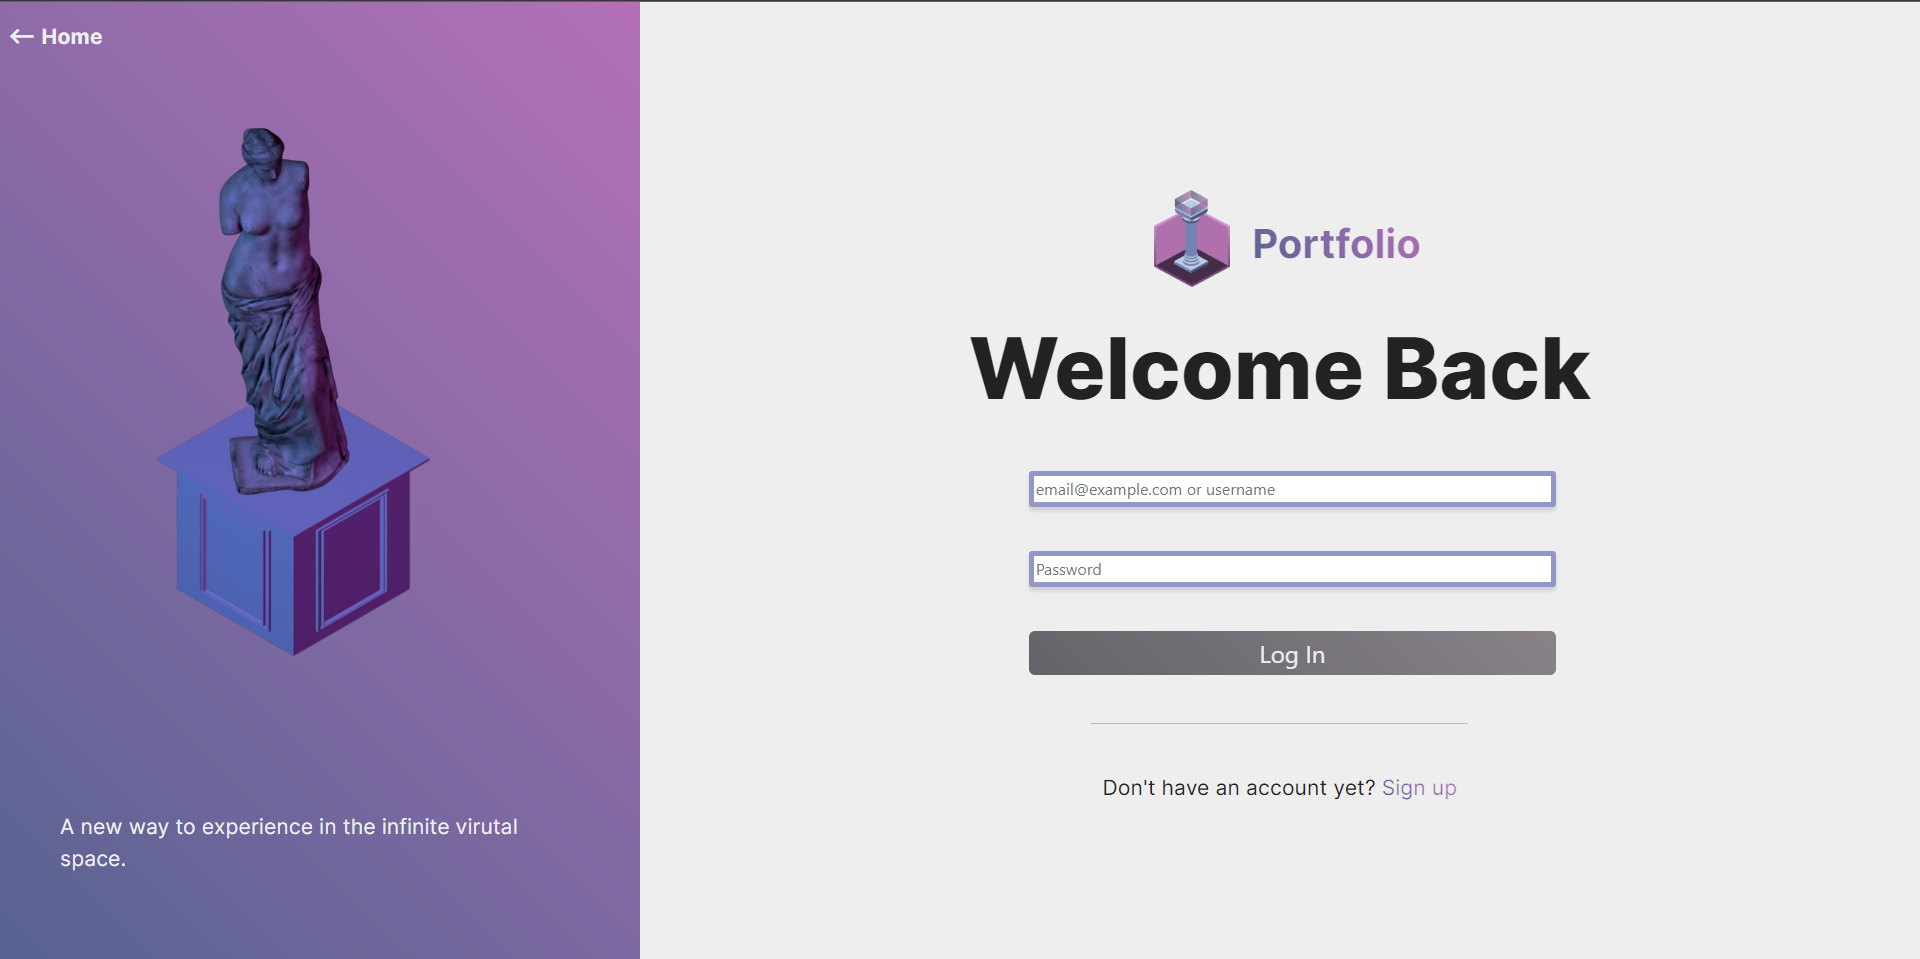
\includegraphics[scale=0.25]{pics/GalleryLogIn.png}
    \caption{Projekt: Login Page}
    \label{fig:impl:login}
\end{figure}

Für das Userinterface wurden Anmelde- und Registrierungs-Funktionalitäten implementiert (siehe Abbildung der Anmeldeseite \ref{fig:impl:login}). Die Anmelde- und Registrationsformulare wurden mithilfe von reaktiven Formularen und Validatoren (siehe Absatz \ref{par:impl:usermanagment:reactiveForms}) umgesetzt. Nachdem eine valide Eingabe von dem*der User*in gemacht wurde, aktiviert sich der Anmelde- bzw. Registrierungsknopf und lässt sich drücken. Die Aktivierung des Knopfes wird durch die Farbveränderung von Grau auf Bunt sichtbar gemacht.  Nachdem der*die User*in die Eingabe bestätigt hatte, indem sie*er den Knopf drückte, werden die Anmeldedaten über das HTTPS-Protokoll mithilfe des HTTP-Moduls (siehe Abschnitt TODO referzieren fabians http-module is not net commitet) an den Server gesendet. Nach einer erfolgreichen Anmeldung / Registration wird an die Weboberfläche eine Antwort geschickt, in der der JWT Token enthalten ist. Danach wird der*die User*in auf die Profilseite weitergeleitet. Bei einer gescheiterten Anmelde- / Registrierungsversuch wird der*die User*in durch eine Fehlermeldung darüber informiert.

Nach der erfolgreichen Anmeldung / Registration wird vom Server ein JWT ausgestellt. Bei einem HTTP-Request vom Client zum Server kann der JWT im Header des Requests platziert werden, der Server kann diesen auslesen und so feststellen, ob ein*e Benutzer*in auch wirklich authentifiziert ist.

Nun gibt es aber mehrere Unbequemlichkeiten, die aus diesem Prozess resultieren. Der*Die User*in muss sich jedes Mal, bei jedem neuen Webseitbesuch und beim neuen Laden der Webseite, neu anmelden und der*die Entwickler*innen müssen bei jedem HTTP-Request (also jeder Kommunikation mit dem Server) manuell den JWT in den Header platzieren.

\paragraph{Formulare und Validation}
\label{par:impl:usermanagment:reactiveForms}
In Webanwendungen gibt es viele Formulare, weil sie dort als eine der primären Kommunikationsschnittstellen zum Besucher*in dienen. Natürlich gibt es dafür den nativen Inputelement von HTML, aber zu einem Formular mit guter Usererfahrung gehört auch ein visuelles Feedback für den*die Benuzter*in, zusätzlich wächst der Entwicklungsaufwand exponentiell mit der Featureanzahl des Formulars.

Angular bietet verschiedene Implementierungsarten, um die visuelle Komponente umzusetzen und den Entwicklungsaufwand zu minimieren. Bei diesen Ansätzen können mehrere Eingabedaten zentral ausgewertet und weiterverarbeitet werden und der Status des Formulars bei Änderungen und Fehlern visuell dargestellt werden.

Bei den Ansätzen kann zwischen den reactive Forms und den Template-Driven-Forms unterschieden werden.

\subparagraph{Template-Driven-Forms}
Bei den Template-Driven-Forms 
TODO template und reactive forms erklären
\cite[Bookmonkey - 12 Formularverarbeitung und
Validierung: Iteration IV]{AngularBuch}

\subsubsection{Token-Verwaltung}
Um das Problem der Anmeldung zu lösen, wurde der JWT im LocalStorage des Browsers gespeichert. Im Codeausschnitt (siehe \ref{lst:impl:sign:jwtLocalstorage}) ist ein Teil des Authentifizierungsdienstes des Projektes zu sehen. Mit der Funktion \emph{setSaveJWT} wird der ausgestellte JWT ausgelesen und die darin enthaltenen Informationen, der Name und die Id des Benutzers, die Id des Tokens und das Ablaufdatum des Tokens im LokalenStorage (siehe im Absatz WebStorage API \ref{par:impl:usermanagment:WebStorage}) gespeichert, damit die Daten auch nach dem Neuladen der Webseite erhalten bleiben. Die Funktion \emph{isLoggedIn} gibt nach dem Aufruf den Status mit, ob eine Person angemeldet ist oder nicht, dafür benutzt die Funktion das im JWT enthaltene Ablaufdatum und vergleicht es mit dem aktuellen Datum. Zuletzt gibt es noch die \emph{logout} Funktion, diese löscht die im LocalStorage enthaltenen JWT-spezifischen Daten.

\begin{lstlisting}[caption=auth.service.ts - JWT und Localstorage,label=lst:impl:sign:jwtLocalstorage,language=TypeScript ]
export class AuthService {
    ...
    setSaveJWT(value: any) {
        let decodedJWTPayload = JSON.parse(atob(value.split('.')[1]))
        localStorage.setItem("user", decodedJWTPayload.sub)
        localStorage.setItem('id_token', value)
        localStorage.setItem('expires_at', decodedJWTPayload.exp)
        localStorage.setItem('user_id', decodedJWTPayload.userid)
      }

    isLoggedIn(): boolean {
        if (localStorage.getItem('id_token') && localStorage.getItem('expires_at')) {
          let temp = new Date().getTime()
          const exp = Number(localStorage.getItem('expires_at'))
          return temp < exp
        } else {
          return false;
        }
      }

    logout() {
        localStorage.removeItem("user")
        localStorage.removeItem('id_token')
        localStorage.removeItem('expires_at')
        localStorage.removeItem('user_id')
      }
    ...
}        
\end{lstlisting}

\paragraph{WebStorage API}
\label{par:impl:usermanagment:WebStorage}
Die WebSotrage API bietet verschiedene Möglichkeiten, Daten per Schlüssel-Werte-Paare im Web zu persistieren. Persistenz ist die Fähigkeit, Daten in einem nicht flüchtigen Speicher zu speichern, um so den Datenverlust beim Neustart des Systems zu verhindern. Die WebStorage API ist nicht Teil des DOM, sondern der globalen Web-Variable window. Die zwei Arten, Daten mittels der WebStorage API zu persistieren, sind der LocalStorage und der SessionStorage.
\cite{WikiPersistenzDefinition} \cite{WebStorageAPI}


\subparagraph{SessionStorage}
Daten im SessionStorage werden je nach ihrem Ursprung getrennt aufbewahrt. Sie werden für die Zeit der Webseitensession gespeichert, wenn der Browser oder der Tab geschlossen wird, sind die Informationen auch fort.
\cite{WebStorageAPI}

\subparagraph{LocalStorage}
Daten werden wie im SessionStorage auch persistiert, doch auch wenn der Browser geschlossen wird bleiben die Daten erhalten. Daten können nur durch JavaScript oder das Löschen des Webbrowser-Caches gelöscht werden.
\cite{WebStorageAPI}

\subparagraph{Allgemeine Informationen}
Beide Speichermethoden benutzen keine Server, um die Daten zu speichern, sondern den Cache des Webbrowsers. Das Speicherlimit hängt vom Webbrowser ab, doch beträgt es meistens 5 MB und es können nur Zeichenketten gespeichert werden.
\cite{WebStorageAPI}

\subsubsection{HTTP-Interceptoren}
HTTP-Interceptoren funktionieren in Angular als Zwischenschicht zwischen den ausgehenden HTTP-Abfragen und den eingehenden HTTP-Antworten und können diese umwandeln.
Das Einsatzgebiet von HTTP-Interceptoren ist bei globalen Änderungen und Funktionen, die an allen HTTP-Requests durchgeführt werden sollen. Es war somit das perfekte Werkzeug, um in allen HTTP-Requests den JWT in den Header zu verpacken.
\cite[10.3 Interceptoren: HTTP-Requests abfangen und transformieren]{AngularBuch}

Wenn ein Request an den Server geht, wird dieser unterbrochen. Es wird überprüft, ob der JWT verfügbar ist. Wenn das zutrifft, wird der ursprüngliche Request geklont, in der Authentifizierungsspalte des Headers wird die JWT-Id hinzugefügt, danach wird der Request wieder zum Server weitergeleitet (siehe Code \ref{lst:impl:sign:JWTInterceptor}). 

\begin{lstlisting}[caption=auth.interceptor.ts - add JWT to Request Header,label=lst:impl:sign:JWTInterceptor,language=TypeScript]
import { Injectable } from '@angular/core';
import {
  HttpRequest,
  HttpHandler,
  HttpEvent,
  HttpInterceptor
} from '@angular/common/http';
import { Observable } from 'rxjs';

@Injectable()
export class AuthInterceptor implements HttpInterceptor {

  constructor() {}

  intercept(request: HttpRequest<unknown>, next: HttpHandler): Observable<HttpEvent<unknown>> {

    const idToken = localStorage.getItem('id_token')
    if (idToken) {
      const cloned = request.clone(
        {
          headers: request.headers.set('Authorization', 'Bearer '.concat(idToken))
        }
      )

      return next.handle(cloned)
    }

    return next.handle(request);
  }
}
\end{lstlisting}

\subsubsection{Routing- und Navigations-Einschränkung}
Zum Start dieses Entwicklungsschrittes war der Interceptor und die JWT Verwaltung fertig. Doch das Projekt brauchte eine besseres visuelles Feedback System um dem*der Kunden*in zu den Anmeldestatus zu zeigen.

Deswegen und um zu verhindern das Benutzer*in auf Unterseiten sind auf denen sie wegen ihres Requistratonstatus (noch nicht authentifiziert) noch nichts machen können, wurde je nach Anmeldestatus andere Routen und Informationen auf der Navigationsbar gezeigt (siehe Abbildung \ref{fig:impl:navbarvergleich}). Dafür wurde die Navigationsleistenlogik und die Navigationsleistenservice angepasst. Zusätzlich wurde AuthGuard verwendet um Routen zu sperren auf, die der*die Benutzer*in wegen dem Requistratonstatus noch keinen Zugriff hat. 

\begin{figure}[h t]
  \centering
  \includegraphics[scale=0.6]{pics/navbarRequistrationsstatusGegenüberstellung.png}
  \caption{Navbar: authentifiziert vs noch nicht authentifiziert}
  \label{fig:impl:navbarvergleich}
\end{figure}

\subsection{Profilepage}
Auf der Profileseite (siehe Abbildung \ref{fig:impl:sign:profile}) sieht der*die Benutzer*in userspezifische Informationen wie den Profilnamen, das Profilfoto, die erstellten Exhibition. Zusätzlich kann der*die Benutzer*in hier neue Ausstellungen anlegen und bereits erstellte Ausstellungen löschen. 

\begin{figure}[h t]
  \centering
  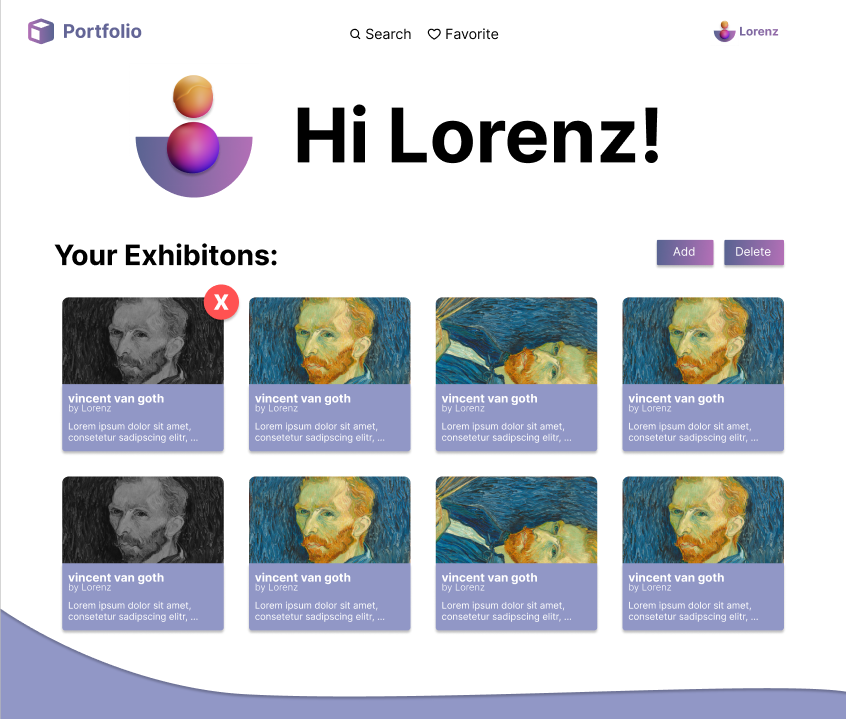
\includegraphics[scale=0.5]{pics/profilepage.png}
  \caption{Profilepage}
  \label{fig:impl:sign:profile}
\end{figure}



\section{Content Creation [L]}
\label{content-creation}
Die Inhaltserstellungs-Funktion ist die Kernfunktion des Projekts. Die Content Creation definiert ein 3D-Portfolio. Ziel ist ein einfacher und intuitiver Konfigurationsprozess für ein 3D-Portfolios. 

\subsection{Datenstruktur}
Die 3D-Ausstellungen lassen sich durch Daten definieren. Die Daten werden bei der Content Creation vom*n Benutzer*in konfiguriert. 

\begin{figure}[ht]
    \centering
    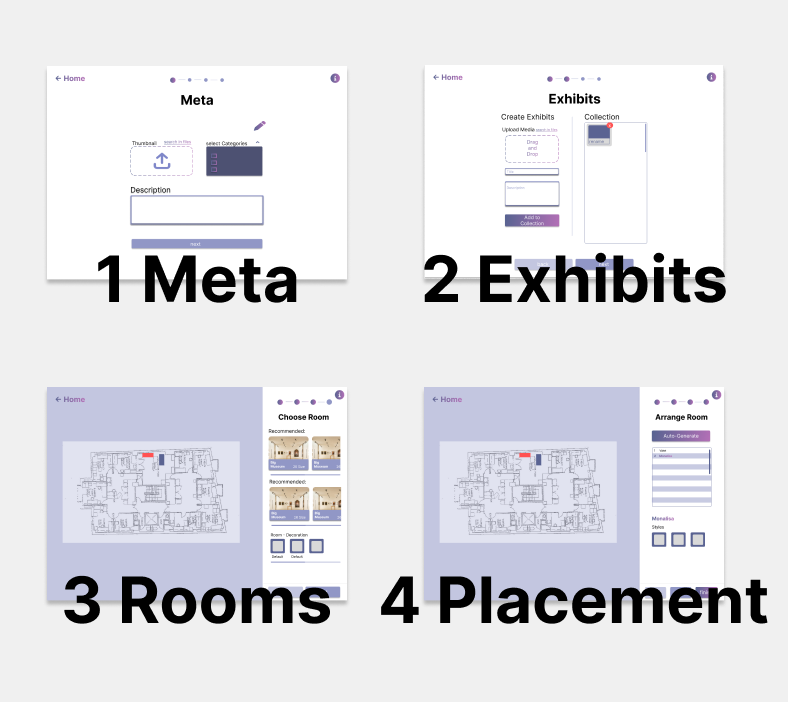
\includegraphics[scale=0.4]{pics/CreateCreation4Categories.png}
    \caption{Inhaltserstellungstool}
    \label{fig:impl:creation:fourCategoires}
\end{figure}

\subsubsection{Kategorie}
\label{sec:wizard:categories}
Die Datenstruktur des Protfolios lässt sich logisch in vier Kategorien (siehe Abbildung \ref{fig:impl:creation:fourCategoires}) teilen. 
Die Kategorien sind:
\begin{compactitem}
\item Metadaten - Die Metadaten sind beschreibende Daten des Portfolio, dazu gehören Name, zugehörige Kategorien, eine Beschreibung und ein Thumbnail.
\item Ausstellungsstücke - Die Ausstellungsstücke werden in dem 3D-Portfolio präsentiert. Die Ausstellungsstücke, Film-, Foto- und 3D Dateien,  werden vom*von Benutzer*in hochgeladen und mit Zusatzinformation wie Namen und Beschreibung ergänzt. 
\item Raumdaten - Raumdaten bestehen aus virtuellen 3D-Daten des Raumes und weiteren Konfigurationsdaten wie den Positionen, an denen Ausstellungsstücke im Raum platziert werden können. Der Grundriss des Raumes kann jede beliebige Form besitzen. 
\item Ausstellungsplatzierungsdaten - Mit diesen Daten werden die Ausstellungsstücke mit dem virtuellen Raum verbunden. Außerdem ist in den Ausstellungsplatzierungsdaten die Dimension eines Ausstellungsstückes enthalten. Jedes Position besitzt eine definierbare Sockelart. 
\end{compactitem}

\paragraph{Ausprägungen}
In der Single-Page-Application werden die vier Kategorien durch Klassen (siehe Abbildung \ref{fig:impl:creation:dataclasses}) definiert. 

\begin{figure}[ht]
    \centering
    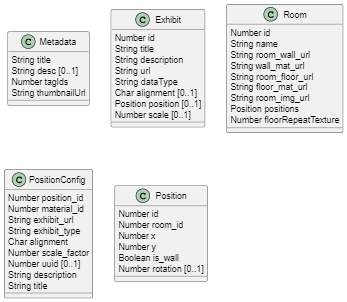
\includegraphics[scale=0.9]{pics/content_creation_classes.png}
    \caption{Inhaltserstellung Datenklassen}
    \label{fig:impl:creation:dataclasses}
\end{figure}

\subsection{GUI}
\subsubsection{Profilepage}
Auf der Profileseite (siehe Abbildung \ref{fig:impl:sign:profile}) sieht der*die Benutzer*in userspezifische Informationen wie den Profilnamen, das Profilfoto und die erstellten Ausstellungen. Zusätzlich kann der*die Benutzer*in hier neue Ausstellungen anlegen und bereits erstellte Ausstellungen löschen.

\begin{figure}
  \centering
  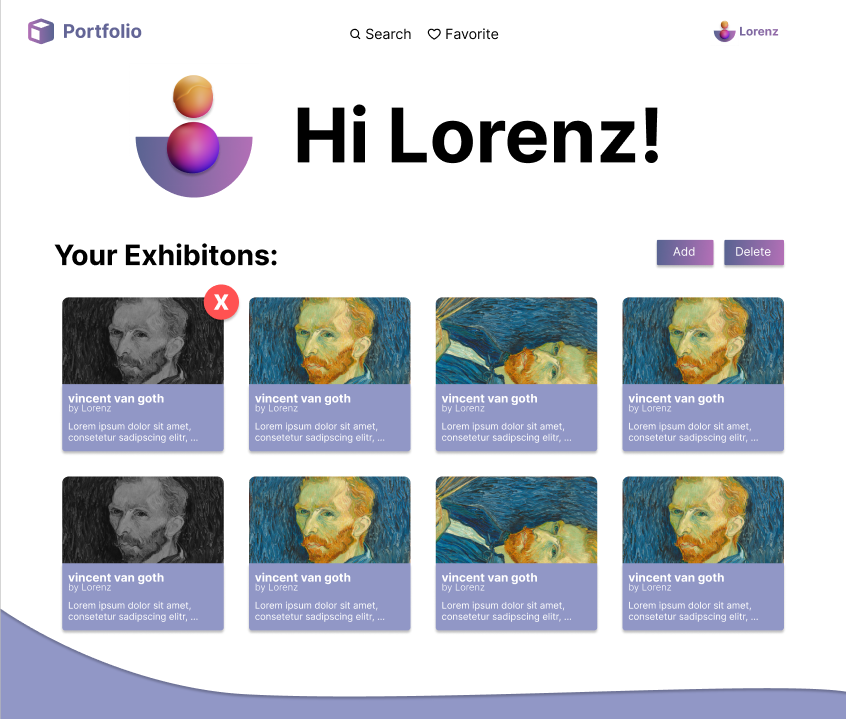
\includegraphics[scale=0.5]{pics/profilepage.png}
  \caption{Profilepage}
  \label{fig:impl:sign:profile}
\end{figure}

\paragraph*{Add Button}
Der Content-Creation-Prozess beginnt damit, dass der "Add-Button" auf der Profileseite gedrückt wird. Danach wird der*die Benutzer*in zu dem Content-Creation-Tool auf der Single-Page-Application weitergeleitet. Dort startet er*sie den Konfigurationsprozess mit dem Metadaten-Formular.


\subsubsection{Formulare}
Die Datensammlung wurde auf vier Formulare, die jeweils einer der vier Datenkategorien (siehe \ref{sec:wizard:categories}) sammeln, aufgeteilt. Das hat das Ziel, dass der*die Benutzer*in sich im Konfigurationsprozess nur mit jeweils einer Portfolio-Daten-Kategorie beschäftigen muss und nicht überfordert wird. Dabei wurde sich am \emph{Wizard-UI-Pattern} (siehe \ref{sec::contentcreation::wizard}) orientiert.


\paragraph{Metadaten-Formulare}
Im Metadaten-Formular werden die Metadaten der Ausstellung gesammelt.


Dabei wurden für die Sammlung der Namen, Beschreibungen und Kategorien der Ausstellung die reaktiven Formulare von Angular und für das Vorschaubild der Ausstellung die eigene Upload-Komponente benutzt. (siehe \ref{sec:wizard:upload}).


\paragraph{Exhibit-Formular}
Im Exhibit-Formular lädt der*die Benutzer*in die gewünschten, die eigenen digitalen Ausstellungsstück hoch.

Diese können nur hochgeladen werden, wenn ihre Datengröße kleiner als 50 MB ist und ihr Filetyp unterstützt wird. Es werden für 3D-Dateien GLTF-Files, für Video-Dateien MP4 und für Photo-Dateien JPG und PNG unterstützt (siehe \ref{sec:wizard:upload})

\paragraph{Raum-Formular}
Im Raumformular wählt der*die User*in zwischen den vordefinierten Grundrissen aus.

In einer 3D-Ansicht neben den Auswahlmöglichkeiten sieht man eine Vorschau, wie der ausgewählte Raum ohne Ausstellungstücke aussieht. 

Abhängig von der Anzahl der hochgeladenen Ausstellungsstücke werden dem*der User*in passende Räume vorgeschlagen.

\paragraph{Ausstellungs-Platzierungs-Formular}
Im Ausstellungs-Platzierungs-Formular werden die hochgeladenen Ausstellungstücke mit dem Grundriss der Ausstellung verbunden.  In einer 3D-Ansicht neben den Auswahlmöglichkeiten sieht man eine Vorschau, wie der Raum mit den Ausstellungstücke aussieht. 

Jeder Grundriss bietet dabei individuelle, im Vorfeld definierte, Positionen. An diesen können Ausstellungsobjekte
platziert werden. Dies kann manuell einzeln oder bei allem automatisiert durchgeführt werden.

Je nach Datentyp des Ausstellungsstückes wird an der Position entweder ein Sockel oder ein Bilderrahmen mit dem Ausstellungstück erschaffen. Der Typ des Sockels und des Bilderrahmens können geändert werden.
Die Größe eines 3D-Ausstellungsstückes wird normalisiert, damit alle Ausstellungstücke gleich groß sind. Dem*der User*in wird die Möglichkeit gegeben, diese Größe noch zu ändern.

\paragraph{Userinterface-Struktur / Wizard Design Pattern [L]}
\label{sec::contentcreation::wizard}
Im Projekt wurde das Wizard-UI-Pattern benutzt, um den Konfigurationsprozess des Portfolios einfacher zu gestalten.

\paragraph*{Wizard Begriffserklärung [L]}
Der Begriff '\emph{Wizard}' in der Softwareentwicklung leitet sich von Systemadministratoren, welche bei komplizierten Installationsprozessen halfen oder ganz übernahmen, ab. Mit der Zeit änderte sich der Begriff zu Software-Assistenz-Applikationen, welche dem*der User*in dabei helfen, die Software zu konfigurieren. \cite[Ursprung des Begriffs Wizard]{OrigionOfWizards}

\paragraph{Wizard-UI-Pattern [L]}
Im Web-Bereich gibt es zwei Arten Dateneintragungen zu verarbeiten: Formulare und Wizards. 
Ein \emph{Wizard} ist eine eigene kleine Applikation, die den*die Benutzer*in durch eine Folge von Formularen führt und gegebenenfalls beim Ausfüllen unterstützt. Je nach Eingabe können Wizards die Formulare passend adaptieren.\cite[Wizards: Definition and Design Recommendations]{WizradsDefinitionAndRecommandation}

\paragraph{Umsetzung des Wizards [L]}
Für die Umsetzung des Wizards wurde die Angular Material Komponente \emph{mat-stepper} benutzt. Sie bietet eine solide Basis für den Wizard. Content kann sequentiell dargestellt werden, während dem*der User*in der aktuelle Status des Wizards durch eine Navigationsleiste angezeigt wird (siehe Abbildung \ref{fig:impl:creation:mathorziontalstepper}). \cite{amStepper}

\begin{figure}
    \centering
    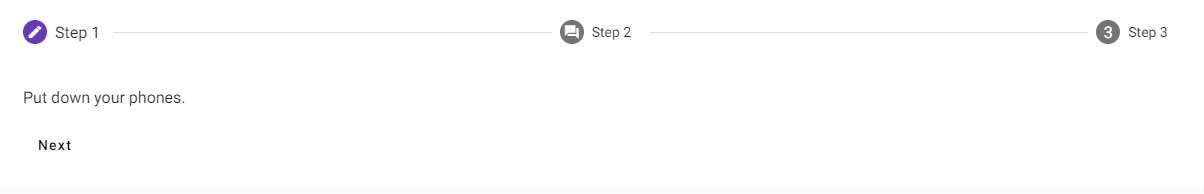
\includegraphics[scale=0.5]{pics/mathorziontalstepper.png}
    \caption{Angular Material: horizontaler Stepper \cite{amStepper}}
    \label{fig:impl:creation:mathorziontalstepper}
\end{figure}

\subsection{Upload}
\label{sec:wizard:upload}
Der Upload-Prozess wurde mit dem Gedanken entwickelt, hoch modular und anpassungsfähig zu sein.

Bei der Komponente sind akzeptable Filetypen und Filegrößen einstellbar. Werden die die gesetzten Anforderungen an Filetypen und Filegrößen von den hochzuladenden Daten nicht erfüllt, so wird der Upload abgebrochen und die Komponente gibt eine Fehlermeldung.
Bei einem erfolgreichen Hochladeprozess bekommt die Komponente eine URL vom Server. Unter der URL ist die hochgeladene Datei erreichbar.

\subsection{Erledigte User-Stories [L]}
In dem Entwicklungsprozess des Content-Creation-Tools wurden folgende User-Stories vollendet:
\begin{compactenum}
    \item  Als User*in will ich eine Profil-Unterseite haben, auf der ich userrelevante Informationen angezeigt bekomme. Dazu gehören der Name, das Profilfoto, und meine erstellten Ausstellungen. Diese möchte ich auch löschen können
    \item Als User*in will ich bei der Erstellung einer Ausstellung zwischen verschiedenen Templates wählen können, um diese auf einfache Weise zu individualisieren - beispielsweise durch die Änderung des Podestes.
    \item Als User*in will ich meine Daten auf den Server laden, um diese jederzeit innerhalb einer Ausstellung platzieren und integrieren zu können. Dazu möchte ich Bilder-, Video-, 3D-Dateien mit einer Größe von maximal 50 MB hochladen können. Bei falschem Upload benötige ich eine Fehlermeldung zur Information.
    \item  Als User*in will ich, dass meine Daten automatisch als Ausstellungsstücke in der Ausstellung angeordnet werden, damit die Nutzung für persönliche Bereiche unkompliziert möglich ist. Falls dies nicht möglich ist, soll eine Fehlermeldung angezeigt werden
    \item Als User*in möchte ich die Reihenfolge und Platzierung meiner Werke innerhalb der Ausstellung adaptieren können. Dazu soll die Wahl zwischen vordefinierten Plätzen möglich sein.
    \item Als User*in möchte ich meine Ausstellung abspeichern und löschen können. 
    \begin{compactitem}
        \item Die Daten im Bezug auf die Ausstellungen werden auf dem Server gespeichert.
        \item Bevor die Ausstellung gelöscht wird, soll ein Warnhinweis angezeigt werden, welcher noch bestätigt werden muss.
    \end{compactitem}
    \item Als Benutzer*in möchte ich meinen Ausstellungen Tags zuordnen können, damit diese leichter gefunden werden können. Dazu soll ein vordefinierter Tag-Pool zur Verfügung stehen, aus welchem ich auswählen kann.
\end{compactenum}

%%\section{3D-Portfolio-Gallery Konfigurationstool [L]} \label{Konfigurationstool}
%%\setauthor{Litzlbauer Lorenz}
%%
%%Die Inhaltserstellung-Funktion ist die Kernfunktion des Projekts. Die Content Creation definiert ein 3D-Portfolio. Ziel ist ein einfacher und intuitiver Konfigurationsprozess für ein 3D-Portfolios. 
%%yyy Im Entwicklungsprozess wurden viele Entscheidungen getroffen, die auf das ganze Projekt Einfluss hatten. Z.B. wurde eine Art der Datenrepräsentation der 3D-Portfolios und die Darstellungsweise der Daten in der 3D-View entwickelt.
%%
%%In diesem Kapitel wird die Softwareentwicklung und der Prozess der Inhaltserstellung erklärt.
%%
%%\begin{figure}
%%    \centering
%%    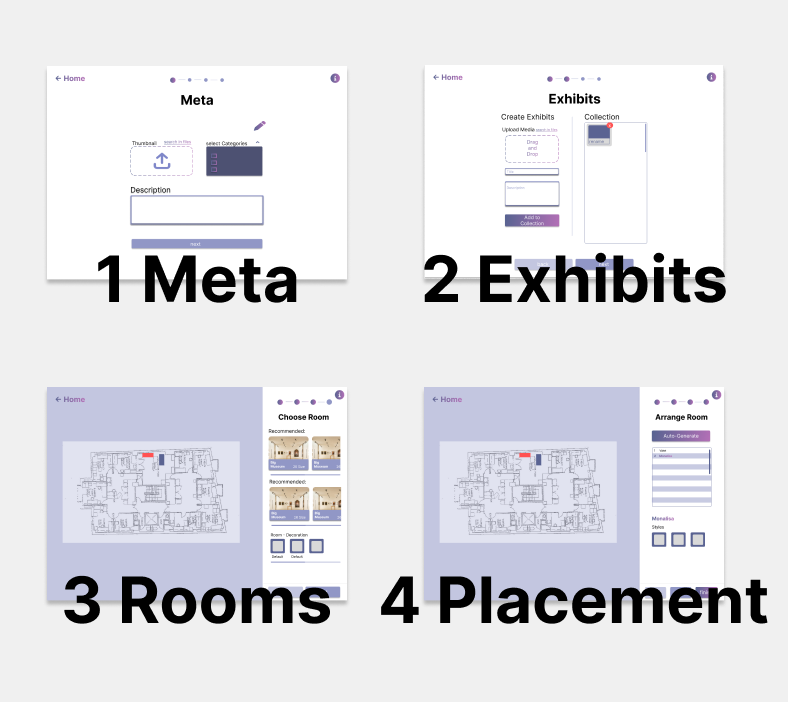
\includegraphics[scale=0.5]{pics/CreateCreation4Categories.png}
%%    \caption{Inhaltserstellungstool}
%%    \label{fig:impl:creation:fourCategoires}
%%\end{figure}
%%
%%\subsection{Überblick [L]}
%%Das Inhaltserstellungs-Tool besteht aus insgesamt vier Bereichen (siehe Abbildung \ref{fig:impl:creation:fourCategoires}), mit diesen werden Daten gesammelt, um das Portfolio zu erstellen und vielen Untersystemen (bestehend aus Komponenten, Klassen und Services siehe Unterkapitel \ref{sec::impl::contentcreation::UnterstuetzendeServicesUndKlassen} auf Seite \pageref{sec::impl::contentcreation::UnterstuetzendeServicesUndKlassen}) , die beim Erstellungsprozess helfen.
%%
%%Diese Unterseiten wurden aufgeteilt, damit der*die Benutzer*in sich im Konfigurationsprozess nur mit jeweils einer Portfolio-Daten-Kategorie beschäftigen muss und nicht überfordert wird. Dabei wurde sich  am \emph{Wizard-UI-Pattern} (mehr dazu im Unterkapitel \ref{sec::contentcreation::wizard} auf der Seite \pageref{sec::contentcreation::wizard}) orientiert.
%%
%%\subsection{Userinterface-Struktur / Wizard Design Pattern [L]}
%%\label{sec::contentcreation::wizard}
%%Im Projekt wurde das Wizard-UI-Pattern benutzt, um den Konfigurationsprozess des Portfolios einfacher zu gestalten. Dafür wurden die Konfigurationsdaten nach 4 Kategorien aufgeteilt und für jede eine eigene Unterseite (siehe Abbildung \ref{fig:impl:creation:fourCategoires}) entworfen.
%%
%%Die Kategorien sind:
%%\begin{compactitem}
%%\item Metadaten - Die Metadaten sind beschreibende Daten für das Portfolio, dazu gehören Name, zugehörige Kategorien, eine Beschreibung und ein Thumbnail.
%%\item Ausstellungsstück - Die Daten des Ausstellungsstücks bestehen aus den vom User auf den Server geladenen Kunstwerken und Zusatzinformation wie Namen und Beschreibung.
%%\item Raumdaten - Raumdaten bestehen aus den virtuellen 3D-Daten des Raumes und weiteren Konfigurationsdaten wie den Positionen, an denen Ausstellungsstücke im Raum platziert werden können.
%%\item Ausstellungsplatzierungsdaten - Mit diesen Daten werden die Daten zu den Ausstellungsstücken und dem virtuellen Raum logisch verbunden.
%%\end{compactitem}
%%
%%\subsubsection*{Begriffserklärung [L]}
%%Der Begriff "\emph{Wizard}" in der Softwareentwicklung, kommt ursprünglich von Systemadministratoren, welche bei komplizierten Installationsprozessen halfen oder ganz übernahmen. Mit der Zeit änderte sich der Begriff zu Software-Assistenten-Programmen, welche dem*der User*in dabei unterstützten, die Software zu konfigurieren. \cite[Ursprung des Begriffs Wizard]{OrigionOfWizards}
%%
%%\subsubsection{Wizard-UI-Pattern [L]}
%%Im Web-Bereich gibt es in der Regel zwei Arten Dateneintragungen zu verarbeiten.
%%
%%Formulare und Wizards. Ein Wizard ist eine eigene kleine Applikation, die den*die Benutzer*in durch eine Folge von Formularen führt und gegebenenfalls beim Ausfüllen unterstützt. Je nach den Eingaben können Wizards die Reihenfolge oder die Formulare ändern.
%%
%%TODO: Bei Bedarf könnte hier mehr geschrieben werden. \cite[Wizards: Definition and Design Recommendations]{WizradsDefinitionAndRecommandation}
%%
%%\subsubsection{Implementation [L]}
%%Für die Implementation des Wizards wurde die Angular Material Komponente Mat-Stepper benutzt. Sie bietet eine solide Basis für den Wizard. Content kann sequentiell dargestellt werden, während dem*der User*in der aktuelle Status des Wizards durch eine Navigationsleiste angezeigt wird (siehe Abbildung \ref{fig:impl:creation:mathorziontalstepper}). \cite{amStepper}
%%
%%\begin{figure}
%%    \centering
%%    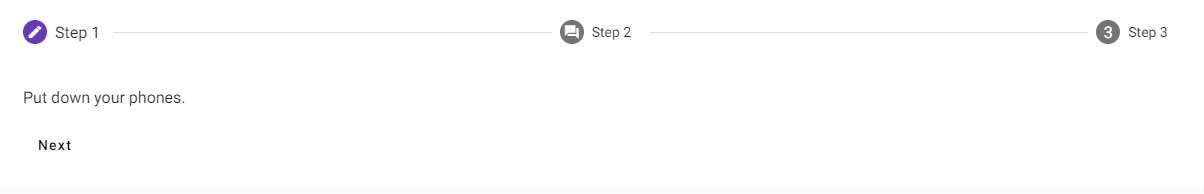
\includegraphics[scale=0.5]{pics/mathorziontalstepper.png}
%%    \caption{Angular Material: horizontaler Stepper \cite{amStepper}}
%%    \label{fig:impl:creation:mathorziontalstepper}
%%\end{figure}
%%
%%\subsection{4 Formularunterseiten [L]}
%%Nachdem die Angular Material Komponente Mat-Stepper für die Wizard-Funktionalität gewählt wurde, war der nächste Schritt, die vier Formularunterseiten des Wizards (siehe Abbildung \ref{fig:impl:creation:fourCategoires}) zu gestalten.
%%
%%In diesem Unterkapitel werden die Funktionalitäten und die Probleme bzw. Lösungen dieser Unterseiten beschrieben. 
%%
%%\subsubsection{Kommunikationsschnittstelle [L]}
%%Die Unterseiten sammeln Daten für die Erstellung des Portfolios. Die Kommunikationsschnittstellen der Unterseiten helfen dabei, dass die Unterseiten miteinander kommunizieren können. Dafür wurde das \emph{Observer-Design-Pattern} (siehe im Glossar \ref{txt:glos:observerDesignPattern} auf Seite \pageref{txt:glos:observerDesignPattern}) gewählt.
%%
%%In einer Dienstklasse, die durch Dependency Injection (siehe Unterkapitel \ref{DPI} auf Seite \pageref{DPI}) mit allen Unterseiten verbunden ist, befinden sich Observablen, die mit den Eingabefeldern der Unterseiten verbunden sind. Wenn auf den Unterseiten eine neue Dateneingabe geschieht, wird die Veränderung an die Dienstklasse weitergegeben. Die Unterseiten haben jeweils eine Datenklasse nach den Kategorien des Portfolios (siehe Abbildung \ref{fig:impl:creation:dataclasses}), in der die Daten gespeichert werden.
%%
%%\begin{figure}
%%    \centering
%%    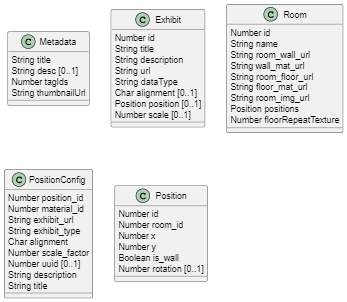
\includegraphics[scale=0.7]{pics/content_creation_classes.png}
%%    \caption{Inhaltserstellung Datenklassen}
%%    \label{fig:impl:creation:dataclasses}
%%\end{figure}
%%
%%In der Dienstklasse werden Veränderungen durch den SessionStorage (siehe Unterkapitel \ref{par:impl:usermanagment:WebStorage} auf Seite \pageref{par:impl:usermanagment:WebStorage}) gespeichert und an den Wizard Mat-Stepper weitergeleitet, um dort den Fortschritt des Konfigurationsprozesses anzuzeigen.
%%
%%Durch die Speicherung im SessionStorage kann der Konfigurationsprozess selbst bei einem Abbruch in der Zukunft nahtlos fortgesetzt werden.
%%
%%\subsubsection{Metadaten - Unterseite [L]}
%%Die Metadaten-Unterseite (siehe Abbildung \ref{fig:impl:creation:Metadaten_Unterseite}) wurde erstellt, um Metadaten wie den Namen, die Kategorien, das Vorschaubild und eine kurze Beschreibung zu der Ausstellung zu sammeln.
%%
%%Alphanumerische Daten wie der Name und die Beschreibung wurden mit Angular's reaktiven Formularen (siehe Kapitel \ref{par:impl:usermanagment:reactiveForms} auf Seite \pageref{par:impl:usermanagment:reactiveForms}) gesammelt.
%%
%%Das Vorschaubild wird hochgeladen mit der Dateien-Hochlade-Komponente (siehe Kapitel \ref{sec:impl:contentcreation:file-Upload} auf Seite \pageref{sec:impl:contentcreation:file-Upload}). Auf der Webapplikation wird die URL gespeichert, unter der die hochgeladene Datei zur Verfügung steht.
%%
%%\begin{figure}
%%    \centering
%%    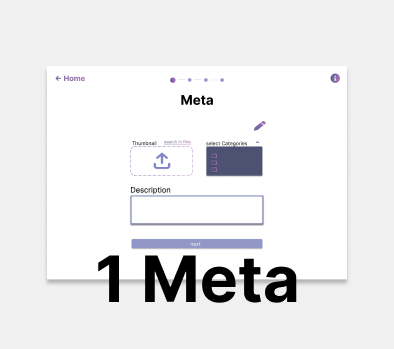
\includegraphics[scale=0.5]{pics/metadaten.png}
%%    \caption{Metadaten Unterseite}
%%    \label{fig:impl:creation:Metadaten_Unterseite}
%%\end{figure}
%%
%%\subsubsection{Ausstelungsstücke - Raum}
%%\subsection{Unterstützende Services und Klassen}
%%\label{sec::impl::contentcreation::UnterstuetzendeServicesUndKlassen}
%%\subsubsection{Dateien-Hochlade-Komponente [L]}
%%\label{sec:impl:contentcreation:file-Upload}
%%
%%TODO: Image vom der Komponente
%%
%%
%%\paragraph{Funktionalitäten und Implementierung [L]}
%%\paragraph{Hochlade Funktionalitäten des Servers [E]}
%%
%%
%%\subsubsection{Portfolio-Veröffentlichung-System [L]}
\section{Border-Collision}
\setauthor{Fabian Maar}

Um den Benutzern und Benutzerinnen ein möglichst realistisches Gefühl für die Ausstellung zu geben, ist es wichtig, den Ausstellungsraum auch so zu gestalten. Daher ist der Raum durch Wände abgegrenzt, wodurch es nicht mehr möglich ist, sich über den Raum hinaus zu bewegen. 
Um eine Kollision mit der Wand zu berechnen, gibt es durch die Three.js Bibliothek einige Möglichkeiten.
\subsection{Erster Ansatz}
Eine davon ist, eine Bounding Box zu erstellen. Dabei unterscheidet man zwischen zwei verschiedenen Arten. Zum einen verwendet man die Axis Aligned Bounding Box, um eine Box rund um das 3D-Objekt zu erstellen, die sich nicht an die Rotation des Objekts anpasst. Die zweite Variante ist die Oriented Bounding Box, die im Endeffekt gleich funktioniert, sich aber darin unterscheidet, dass sie sich an die Achsen des Objekts anpasst. Da sich die Bounding Boxen jedoch über das ganze 3D-Objekt erstrecken, wird eine Kollision direkt berechnet, nachdem der*die Benutzer*in den Raum betritt. Da sich die Bounding Boxen nicht an jede einzelne Wand anpassen konnten, musste ein anderer Lösungsweg gefunden werden.

\begin{figure}
    \centering
    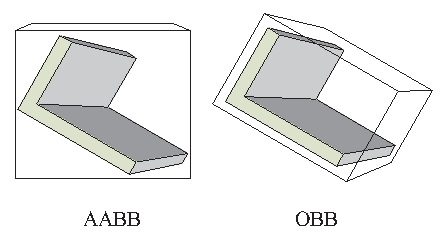
\includegraphics[scale=0.65]{pics/aabb_obb.png}
    \caption{Der Unterschied zwischen AABB und OBB}
    \label{fig:impl:aabb_obb}
\end{figure}

\subsection{Zweiter Ansatz}
Um eine Veränderung der Position des*der Benutzers*in festzustellen, muss die Veränderung der Kameraposition evaluiert werden. Dabei wird beim initialisieren der Kamera eine Kopie von ihr erstellt. In der Animate-Funktion wird eine Veränderung der Kamera überprüft, indem die Positionen der Kamera mit der Kopie verglichen werden. Die Kamera nimmt dabei immer eine neue Position ein, wenn sich der*die Benutzer*in im Raum bewegt, während die Kopie dabei die alte Position der Kamera einnimmt.    
Jedesmal wenn eine Veränderung geschieht, wird überprüft, ob die Kamera mit der Wand kollidiert. Dies geschieht, indem ein Raycast mit den Positionen der Kamera und der Kopie initialisiert wird. 
\subsection{Far und Near}
Die Attribute Far und Near werden dafür verwendet, um die Objekte, die im Ray liegen, einzugrenzen. Dabei können die Werte nicht negativ sein und der Far-Wert muss größer als der Near-Wert sein. Um die Kollision erst direkt am Ursprungsort, im Falle der Kamera, des Rays zu berechnen, wird der Far-Wert auf 100 gesetzt.
   	
Nachdem der Raycast korrekt initialisiert und angewandt wurde, muss bei einer Berührung mit der Wand nur noch richtig damit umgegangen werden. Dabei wird die Bewegung des Benutzers gestoppt. Um diese auch wieder zu starten, muss sich der*die Benutzer*in weg von der Wand begeben. Überprüft wird dies nach jeder Benutzer*inneneingabe mit einem Event-Listener. Falls nach dieser keine Berührung mehr mit einer Wand besteht, wird die Bewegung fortgesetzt und der*die Besucher*in kann sich wieder frei im Raum bewegen.
\newpage



